%+++++++++++++++++++++++++++++++++++++++++++++++++++++++++++++++++++++
%Projeto pedagógico do Curso de Engenharia Eletrônica da Universidade Tecnológica Federal do Paraná (UTFPR) - Campus Toledo
%Baseado nas orientações do estilo abntex2 (http://linorg.usp.br/CTAN/macros/latex/contrib/abntex2/doc/abntex2.pdf)
%Autor: Núcleo Docente Estruturante 
% Contato: Prof. Felipe Walter Dafico Pfrimer - pfrimer@utfpr.edu.br
%Ultima atualização: 03/02/2021
%
%+++++++++++++++++++++++++++++++++++++++++++++++++++++++++++++++++++++
%Tipo de documento ABNTEX2:
\documentclass[12pt,openright,oneside,a4paper,
%sumario=tradicional, % para o recomendado pela ABNT utilize sumario=abnt-6027-2012
sumario=abnt-6027-2012,
chapter=TITLE,  % títulos de capítulos convertidos em letras maiúsculas
section=TITLE,  % títulos de seções convertidos em letras maiúsculas
subsection=TITLE, % títulos de subseções convertidos em letras maiúsculas
subsubsection=TITLE, % títulos de subsubseções em letras maiúsculas
subsubsubsection=TITLE, % títulos de subsubsubseções em letras maiúsculas
english,french,spanish,brazil]{abntex2}
%Observe que a ABNT NBR 14724:2011 (seção 5.1) recomenda que os documentos sejam impressos no anverso e no verso das folhas. Isso é obtido com a opção twoside.

%+++++++++++++++++++++++++++++++++++++++++++++++++++++++++++++++++++++
%Pacotes para língua portuguesa do Brasil (código recomendado pelo estilo abntex2):
\usepackage{ifxetex}
\ifxetex
    \usepackage{fontspec}
    \defaultfontfeatures{Ligatures={TeX}}
\else
    \usepackage[utf8]{inputenc}
    \usepackage[T1]{fontenc}
\fi

%Observação: Quando um documento é compilado com xelatex, os pacotes inputenc e fontenc não devem ser incluídos ao preâmbulo do documento. Ao invés desses pacotes, geralmente fontspec é usado. O código anterior de preâmbulo torna flexível a compilação do documento, que pode tanto ser realizada da forma tradicional com pdflatex quanto com xelatex, uma vez que inclui seletivamente os pacotes adequados para cada compilador (página 14 do link http://linorg.usp.br/CTAN/macros/latex/contrib/abntex2/doc/abntex2.pdf).

% Editar o documento "dados_gerais.tex" com as informações do curso
%+++++++++++++++++++++++++++++++++++++++++++++++++++++++++++++++++++++
%Informações do PPC:
\titulo{Projeto Pedagógico do Curso de Engenharia Eletrônica}
\autor{Núcleo Docente Estruturante}
\data{\the\year} % Apenas o ano
\local{Toledo} % Apenas a cidade
\instituicao{Universidade Tecnológica Federal do Paraná
    \par
    Pró-reitoria de graduação e Educação Profissional
    \par
    Campus Toledo}
\tipotrabalho{Projeto Pedagógico do Curso de Engenharia Eletrônica}


%+++++++++++++++++++++++++++++++++++++++++++++++++++++++++++++++++++++
%Preambulo (Texto apresentado na contracapa):

\preambulo{Projeto Pedagógico de Curso apresentado ao Conselho de Graduação e Educação Profissional - COGEP da UTFPR e aprovado pela Resolução \pdfmarkupcomment{COGEP XXX, DE XX/XX/20XX}{Inserir depois de aprovado, ou considerar a primeira aprovação pelo COGEP}}



% Formatação da capa

\renewcommand{\imprimircapa}{%
    \begin{capa}%
        \center
        
\includegraphics[width=3cm]{brasao.eps}
        
        \ABNTEXchapterfont\Large \imprimirinstituicao
        
        \vspace*{1cm}
        
        %{\ABNTEXchapterfont\large\imprimirautor}
        
        \vfill
        \begin{center}
            \ABNTEXchapterfont\bfseries\LARGE\imprimirtitulo
        \end{center}
        \vfill
        
        \large\imprimirlocal
        
        \large\imprimirdata
        
        \vspace*{1cm}
    \end{capa}
}

%+++++++++++++++++++++++++++++++++++++++++++++++++++++++++++++++++++++
%Pacotes adicionais:
\usepackage{amssymb}
\usepackage{tabto}

\usepackage[%
    %alf,
    num,
    abnt-emphasize=bf,
    bibjustif,
    recuo=0cm,
    abnt-url-package=url,       % Utiliza o pacote url
    abnt-refinfo=yes,           % Utiliza o estilo bibliográfico abnt-refinfo
    abnt-etal-cite=3,
    abnt-etal-list=3,
    abnt-thesis-year=final
]{abntex2cite} 
\usepackage[pdftex]{color,graphicx}
%\usepackage{graphicx}
\usepackage[author=Pfrimer,markup=Highlight,color=yellow]{pdfcomment}
\usepackage[table,xcdraw]{xcolor}
\usepackage{nomencl} % Para a lista abreviaturas e siglas
\makenomenclature    % Para a lista abreviaturas e siglas

% Remove o título original da Nomeclatura:
\renewcommand{\nomname}{}
% Modifica a separação do itens:
\setlength{\nomitemsep}{0pt}
\setlength{\nomlabelwidth}{2.5cm}
% Definição do grupos:
\RequirePackage{ifthen}
 \renewcommand{\nomgroup}[1]{%
     \ifthenelse{\equal{#1}{A}}{\cleardoublepage\item\makebox[0.8\linewidth]{\textbf{\uppercase{\large{Lista de Abreviaturas e Siglas}}}} \makebox[\linewidth]{}\\[0.6cm]}{%
     \ifthenelse{\equal{#1}{S}}{\cleardoublepage\item\makebox[0.8\linewidth]{\textbf{\uppercase{\large{Lista de Símbolos}}}} \makebox[\linewidth]{}\\[0.6cm]}{}}}

\usepackage{indentfirst} % Indenta o primeiro parágrafo de cada seção.
\usepackage{multirow} % Pacote de tabulação para tabelas
\usepackage{bm} % Define o comando \bm para cujo argumento fica em negrito, inclusive formulas matemáticas
\usepackage{lastpage} % Usado por abntex2-fichacatalografica.tex
\usepackage[font=small,labelfont=bf,textfont=bf]{caption} % Legendas de floats em tamanho 10pt e negrito
\usepackage{listings} % Permite digitar códigos em Latex
\usepackage{textcomp} % Pacote com símbolos adicionais para latex (Ex.: baht, bullet, copyright, musicalnote, onequarter, section e yen)
\usepackage{caption} % Permite customizar a legenda de figuras e tabelas
\usepackage{upgreek} % Utilizado para letras gregas não-itálicas
\usepackage{lscape} % Permite rotacionar páginas, mas não os números das páginas.
\usepackage{lipsum} % Para texto filler
\usepackage{verbatim}
\usepackage{listings}
\usepackage{pgfgantt}
%\usepackage[a-1b]{pdfx}

\usepackage{hyperref}

%insira novos pacotes aqui:

\usepackage{pgfplotstable} % Permite criar tabelas com arquivos csv
\usepackage{booktabs} % Estilos de linha para tabelas
\usepackage{enumitem} % Para formatar as listas
\usepackage{multicol} % Mesclar colunas em tabelas
\usepackage{multirow} % Mesclar linhas em tabelas
\usepackage{eurosym}
\usepackage{pdflscape}
\usepackage{colortbl}
\usepackage{cellspace}
\setlength\aboverulesep{0pt}
\setlength\belowrulesep{0pt}
\setlength\cellspacetoplimit{3pt}
\setlength\cellspacebottomlimit{3pt}
\usepackage{bigstrut}
\usepackage{makecell}
\renewcommand\theadalign{bc}
\renewcommand\theadfont{\bfseries}
\renewcommand\theadgape{\Gape[4pt]}
\renewcommand\cellgape{\Gape[4pt]}


%+++++++++++++++++++++++++++++++++++++++++++++++++++++++++++++++++++++
%Outras configurações:

% "Por padrão, uma versão sem serifas da fonte corrente do documento é utilizada para os títulos das divisões. Você pode customizar a fonte dos títulos dos capítulos alterando os comandos como no exemplo a seguir, para que seja utilizada a fonte Computer Modern com tamanho maior do que o utilizado por padrão" (manual do abntex2).
\renewcommand{\ABNTEXchapterfont}{\fontfamily{cmr}\fontseries{b}\selectfont}
\renewcommand{\ABNTEXchapterfontsize}{\large}
\renewcommand{\ABNTEXsectionfontsize}{\normalsize}
\renewcommand{\ABNTEXsubsectionfontsize}{\normalsize}
\renewcommand{\ABNTEXsubsubsectionfontsize}{\normalsize}
\renewcommand{\ABNTEXsubsubsubsectionfontsize}{\normalsize}

% Para criação de quadros
% Novo list of (listings) para QUADROS:
\newcommand{\quadroname}{Quadro}
\newcommand{\listofquadrosname}{Lista de quadros}

\newfloat[chapter]{quadro}{loq}{\quadroname}
\newlistof{listofquadros}{loq}{\listofquadrosname}
\newlistentry{quadro}{loq}{0}

% configurações para atender às regras da ABNT (não remover ou alterar) 
\setfloatadjustment{quadro}{\centering}
\counterwithout{quadro}{chapter}
\renewcommand{\cftquadroname}{\quadroname\space} 
\renewcommand*{\cftquadroaftersnum}{\hfill--\hfill}

% Configuração de posicionamento padrão:
\setfloatlocations{quadro}{hbtp}


%\setlength\afterchapskip{\lineskip} % Espaçamento de 1,5 entre o título do capítulo e corpo do texto

% informações do PDF
\makeatletter
\hypersetup{
	%pagebackref=true,
	%pdftitle={Teste}, 
	%pdfauthor={\imprimirautor},
	%pdfsubject={\imprimirpreambulo},
	%pdfcreator={LaTeX with abnTeX2},
	%pdfkeywords={abnt}{latex}{abntex}{abntex2}{livro}, 
	colorlinks=true,       		% false: boxed links; true: colored links
	linkcolor=blue,          	% color of internal links
	citecolor=blue,        		% color of links to bibliography
	filecolor=magenta,      		% color of file links
	urlcolor=blue,
	bookmarksdepth=4
}
\makeatother
% ---
\makeatletter
\pdfinfo {   
	/Title (teste)
	/Author (teste)
	/Subject (teste)
	/Keywords (teste) 
}
\makeatother

% comandos customizados

\newcommand{\utf}{Universidade Tecnológica Federal do Paraná}

%+++++++++++++++++++++++++++++++++++++++++++++++++++++++++++++++++++++
%Início do documento:
\begin{document}
    %+++++++++++++++++++++++++++++++++++++++++++++++++++++++++++++++++
    % Elementos pré-textuais
    \pretextual

    % Imprime capa e pula sua numeração
    \pagenumbering{gobble} % Remove a visualização da numeração das páginas e reinicia em 1 
    \clearpage
    \thispagestyle{empty}
    \imprimircapa
    \clearpage
    \pagenumbering{arabic}% Numeração arábica (e reinicia em 1)

    % Imprime a folha de rosto (padrão do abntex2)
    \imprimirfolhaderosto*

    %Lista de figuras
    \pdfbookmark[0]{\listfigurename}{lof}
    \listoffigures* 
    \cleardoublepage

    %Lista de tabelas (Opcional)
    %\listoftables

    %lista de abreviaturas e siglas
    \pdfbookmark[0]{\nomname}{lst}
    \printnomenclature
    \cleardoublepage

    %Sumário
    \pdfbookmark[0]{\contentsname}{toc}
    \tableofcontents*
    \cleardoublepage
    
    %+++++++++++++++++++++++++++++++++++++++++++++++++++++++++++++++++
    \chapter*{Pendências}

\section*{Geral}

\begin{itemize}
 	\item Mudar a palavra disciplina para ``unidade curricular''?
\end{itemize}

\section*{Capítulos 1 e 2}

\begin{itemize}
	\item Estão sob revisão do Nakano e Marcos (01/04/2021)
\end{itemize}

\section*{Capítulo 3}

\begin{itemize}
	\item A \autoref{sec:artc} foi copiada do PCC atual, precisa verificar se está atualizado em relação às novas DCNs. Também precisa verificar as porcentagens de aulas práticas (o texto está destacado em amarelo);
	\item A \autoref{sec:desen}, que trata das competências, precisa ser atualizada para a DCN atual;
	\item A \autoref{sec:flex} precisa ser revisada, remover ou modificar os parágrafos grifados em amarelo;
\end{itemize}

\section*{Capítulo 4}

\begin{itemize}
	\item Atualizar quantitativo de engenheiros no Brasil. Estudo apontam que etá sobrando profissionais, mas falta os bons, aqueles que são melhores qualificados. \href{https://sites.usp.br/lgi/em-tres-anos-numero-de-engenheiros-formados-ja-supera-em-25-vezes-demanda-prevista-para-2020/}{clique aqui para a fonte.}
	\item Resumir a \autoref{sec:obj};
	\item Na \autoref{sec:perf}, verificar se mantemos o texto feito durante o desing de cursos;
\end{itemize}

\section*{Capítulo 5}

Complementar de acordo com o texto norteador

\begin{itemize}
	\item 
\end{itemize} % Pendências do documento
    % Elementos textuais
    \textual
    
    
    %\chapter{CAPÍTULO, NÍVEL 1}
\label{chap:nivel1}

    Toda seção deve conter um corpo de texto, obrigatoriamente. Insira um novo capítulo com o comando \verb|\chapter{<título>}|, substituindo \verb|<título>| pelo título do capítulo. Use o comando \verb|label{<chave>}| logo após \verb|\chapter{}| para utilizar referência cruzada. O \autoref{qua:intro} mostra um exemplo de código. Observação: se utilizar o sumário tradicional (veja a declaração \verb|\documentclass[]{}| no arquivo \verb|main.tex|) escreva o título capitalizado para garantir que os títulos fiquem em maiúsculo no sumário. Essa observação também é válida para seções e subseções.
    
\begin{quadro}[!htb]
    \centering
    \caption{Exemplo de novo capítulo \label{qua:intro}}
    \begin{tabular}{|c|l|}
        \hline
        1 &\verb|\chapter{Introdução}|\\
        2 &\verb|\label{chap:intro}|\\
        3 &\\
        4 &\verb|<texto>|\\
        \hline
    \end{tabular}
    \fonte{Autoria própria}
\end{quadro}

\nomenclature[S]{$T_S$}{Temperatura}
\nomenclature[S]{$X_i$}{Ponto inicial}

\section{SEÇÃO, NÍVEL 2}
\label{sec:nivel2}

    Essa é uma seção, nível 2, do \autoref{chap:nivel1}. Utilize o comando \verb|\section{<título>}| para criar uma nova seção de nível 2. O \autoref{qua:sec} mostra um exemplo de código.
    
    \begin{quadro}[!htb]
    \centering
    \caption{Exemplo de nova seção de nível 2 \label{qua:sec}}
    \begin{tabular}{|c|l|}
        \hline
        1 &\verb|\section{A vida da marmota}|\\
        2 &\verb|\label{sec:marm}|\\
        3 &\\
        4 &\verb|<texto>|\\
        \hline
    \end{tabular}
    \fonte{Autoria própria}
    \end{quadro}
    
\subsection{SUBSEÇÃO, NÍVEL 3}
\label{subsec:nivel3}

    Essa é uma subseção, nível 3, da \autoref{sec:nivel2}. Caso seja necessário criar uma seção desse tipo em seu texto, utilize o comando \verb|\subsection{<título>}| para criar uma nova seção de nível 3. O \autoref{qua:subsec} mostra um exemplo de código.
    
    \begin{quadro}[!htb]
    \centering
    \caption{Exemplo de nova seção de nível 3 \label{qua:subsec}}
    \begin{tabular}{|c|l|}
        \hline
        1 &\verb|\subsection{Onde vivem}|\\
        2 &\verb|\label{sec:viva}|\\
        3 &\\
        4 &\verb|<texto>|\\
        \hline
    \end{tabular}
    \fonte{Autoria própria}
    \end{quadro}
    
\subsubsection{SUBSEÇÃO, NÍVEL 4}
\label{subsubsec:nivel4}

    Essa é uma subseção, nível 4, da \autoref{subsec:nivel3}. Caso seja necessário criar uma seção desse tipo em seu texto, utilize o comando \verb|\subsubsection{<título>}| para criar uma nova seção de nível 4. O \autoref{qua:subsubsec} mostra um exemplo de código.
    
    \begin{quadro}[!htb]
    \centering
    \caption{Exemplo de nova seção de nível 4 \label{qua:subsubsec}}
    \begin{tabular}{|c|l|}
        \hline
        1 &\verb|\subsubsection{O que comem}|\\
        2 &\verb|\label{sec:food}|\\
        3 &\\
        4 &\verb|<texto>|\\
        \hline
    \end{tabular}
    \fonte{Autoria própria}
    \end{quadro}
    
\subsubsubsection{SUBSEÇÃO, NÍVEL 5}
\label{subsubsubsec:nivel5}

    Isso é uma subseção, nível 5, da \autoref{subsubsec:nivel4}. Pela norma da Associação Brasileira de Normas Técnicas (ABNT), \nomenclature[A]{ABNT}{Associação Brasileira de Normas Técnicas} subseções são permitidas até o nível 5 \cite{NBR6024:2012}. Caso seja necessário criar uma seção desse tipo em seu texto, utilize o comando \verb|\subsubsubsection{<título>}| para criar uma nova seção de nível 5. O \autoref{qua:subsubsubsec} mostra um exemplo de código.
    
    \begin{quadro}[!htb]
    \centering
    \caption{Exemplo de nova seção de nível 5 \label{qua:subsubsubsec}}
    \begin{tabular}{|c|l|}
        \hline
        1 &\verb|\subsubsubsection{Como se reproduzem}|\\
        2 &\verb|\label{sec:sex}|\\
        3 &\\
        4 &\verb|<texto>|\\
        \hline
    \end{tabular}
    \fonte{Autoria própria}
    \end{quadro}
    
\section{SIGLAS, ACRÔNIMOS E SÍMBOLOS}
\label{sec:siglas}

    Para acrescentar uma sigla ou acrônimo na lista de siglas e acrônimos utilize o comando \verb|\nomenclature[A]{<sigla>}{<significado>}| em qualquer parte do texto. É recomendado inserir esse comando logo após a primeira aparição da sigla ou do acrônimo. Um exemplo de código está transcrito no \autoref{qua:siglacode}. 
    
    \begin{quadro}[!htb]
    \centering
    \caption{Exemplo de código para a acrescentar siglas ou acrônimos na lista \label{qua:siglacode}}
    \begin{tabular}{|l|}
        \hline
        \makebox[0.9\linewidth]{\textbf{Código}}\\
        \hline
        \verb|A Ordem dos Advogados do Brasil (OAB) \nomenclature[A]{OAB}{Ordem dos|\\
        \verb|Advogados do Brasil} diz que apoia investigação do ataque de milícias|\\
        \verb|digitais ao Supremo Tribunal Federal (STF) \nomenclature[A]{STF}|\\
        \verb|{Supemo Tribunal Federal}.|\\
        \hline
        \hline
        \makebox[0.9\linewidth]{\textbf{Resultado}}\\
        \hline
        A Ordem dos Advogados do Brasil (OAB) \nomenclature[A]{OAB}{Ordem dos|Advogados do Brasil} diz que apoia investigação do ataque de \\
        milícias digitais ao Supremo Tribunal Federal (STF) \nomenclature[A]{STF}{Supemo Tribunal Federal}.\\
        \hline
    \end{tabular}
    \fonte{Autoria própria}
    \end{quadro}
    
    
    
    
    Para acrescentar um símbolo na lista de símbolos utilize o comando \verb|\nomenclature[S]| \verb|{<simbolo>}{<significado>}| em qualquer parte do texto. É recomendado inserir esse comando logo após a primeira aparição do símbolo. Um exemplo de código está transcrito no \autoref{qua:simbcode}.
    
    \begin{quadro}[!htb]
    \centering
    \caption{Exemplo de código para a acrescentar símbolos na lista \label{qua:simbcode}}
    \begin{tabular}{|l|}
        \hline
        \makebox[0.9\linewidth]{\textbf{Código}}\\
        \hline
        \verb|A segunda lei de Newton diz que $F_r = ma$, onde $F_r$|\\
        \verb|\nomenclature[S]{$F_r$}{Força resultante} é a força resultante, $m$|\\
        \verb|\nomenclature[S]{$m$}{massa} é a massa e $a$ \nomenclature[S]{$a$}|\\
        \verb|{aceleração} é a aceleração.|\\
        \hline
        \hline
        \makebox[0.9\linewidth]{\textbf{Resultado}}\\
        \hline
        A segunda lei de Newton diz que $F_r = ma$, onde $F_r$ \nomenclature[S]{$F_r$}{Força resultante} é a força resultante,\\
        $m$ \nomenclature[S]{$m$}{massa} é a massa e $a$ \nomenclature[S]{$a$}{aceleração} é a aceleração.\\
        \hline
    \end{tabular}
    \fonte{Autoria própria}
    \end{quadro}
    
    Para que as listas sejam geradas é necessário que o comando \textit{\textbf{makeindex}} seja executado com os seguintes argumentos: 
    
    \makebox[0.95\linewidth]{makeindex -s nomencl.ist -o main.nls main.nlo}
    
    \noindent onde ``main'' é o nome do arquivo principal do projeto. Procure mais informações na base de dados do seu editor e copilador \LaTeX.
    
    
\section{SOBRE AS REFERÊNCIAS CRUZADAS E ITENS NUMERADOS}
\label{sec:refs}

    A numeração sequencial de figuras, tabelas, quadros e equações ocorre de modo automático. As ilustrações (figuras), tabelas e quadros serão indexadas automaticamente em suas respectivas listas. 

    Referências cruzadas são obtidas através dos comandos \verb|\label{}| e \verb|\ref{}|. Sendo assim, não é necessário por exemplo, saber que o número de certo capítulo para colocar o seu número no texto. O comando \verb|\autoref{}| facilita referenciação de elementos numerados no texto sem a necessidade de nomear o tipo do elemento.
    
    Observe que este capítulo recebeu a chave ``chap:nivel1'' através do comando \verb|\label{}| (\verb|\label{chap:nivel1}|). Dessa forma, ao utilizar o código \verb|\ref{chap:nivel1}| resulta na escrita do número do capítulo que nesse caso é ``\ref{chap:nivel1}''. De forma análoga, o comando \verb|\autoref{chap:nivel1}| resulta em ``\autoref{chap:nivel1}''.
    
\section{FIGURAS}
\label{sec:figuras}

    Esta seção trata de um exemplo de como inserir uma figura. Note que a \autoref{fig:figura-exemplo1} aparece automaticamente na lista de figuras. Para saber mais sobre o uso de imagens no \LaTeX{} consulte literatura especializada \cite{Goossens2007}.

    \begin{figure}[!htb]
        \centering
        \caption{Exemplo de Figura}
        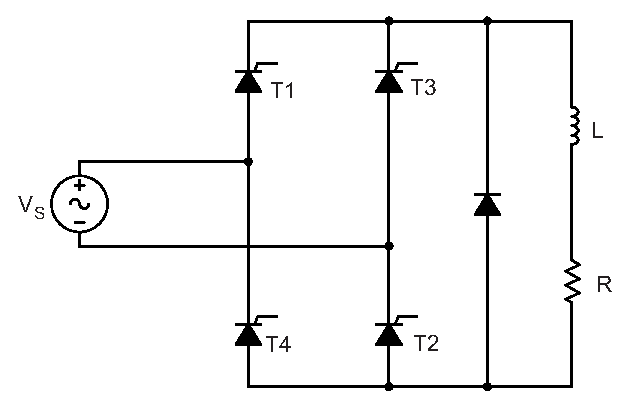
\includegraphics[width=0.6\textwidth]{Caps/Figs/exemplo.eps}
        \fonte{Autoria Própria}
        \label{fig:figura-exemplo1}
    \end{figure}
    
    O código utilizado para inserir a \autoref{fig:figura-exemplo1} está listado no \autoref{qua:figura}.
    
    \begin{quadro}[!htb]
    \centering
    \caption{Código exemplo utilizado para inserir a \autoref{fig:figura-exemplo1} \label{qua:figura}}
    \begin{tabular}{|c|l|}
        \hline
        1 &\verb|\begin{figure}[!htb]|\\
        2 &\verb|\centering|\\
        3 &\verb|\caption{Exemplo de Figura}|\\
        4 &\verb|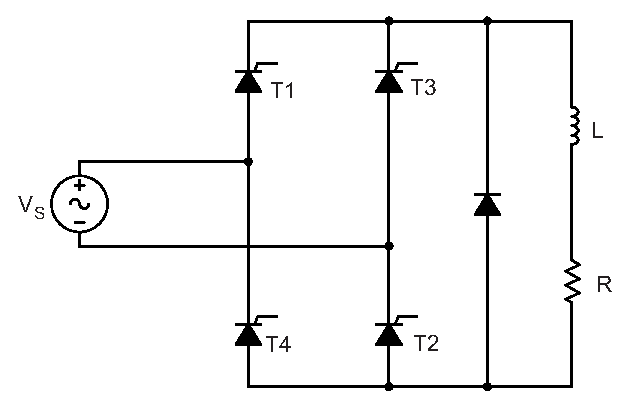
\includegraphics[width=0.6\textwidth]{Caps/Figs/exemplo.eps}|\\
        5 &\verb|\fonte{Autoria Própria}|\\ 
        6 &\verb|\label{fig:figura-exemplo1}|\\ 
        7 &\verb|\end{figure}|\\ 
        \hline
    \end{tabular}
    \fonte{Autoria própria}
    \end{quadro}
    
    Utilize figuras no formato \textit{Encapsulated PostScript} (EPS)\nomenclature[A]{EPS}{\textit{Encapsulated PostScript}}. Caso precise de outro formato, acrescente no preambulo deste modelo o pacote adequado para a sua necessidade.
    
\section{QUADROS E TABELAS}
\label{sec:tabelas}

    Esta seção trata de exemplos de como inserir o \autoref{qua:quadro-exemplo1} e a \autoref{tab:tabela-exemplo1}. Ambos aparecem automaticamente nas suas respectivas listas. Para saber mais informações sobre a construção de tabelas no \LaTeX{} consulte literatura especializada \cite{Mittelbach2004}.

    \begin{quadro}[!htb]
    \centering
    \caption{Exemplo de Quadro \label{qua:quadro-exemplo1}}
    \begin{tabular}{|p{7cm}|p{7cm}|}
        \hline
        \textbf{BD Relacionais} & \textbf{BD Orientados a Objetos} \\
        \hline
        Os dados são passivos, ou seja, certas operações limitadas podem ser automaticamente acionadas quando os dados são usados. Os dados são ativos, ou seja, as solicitações fazem com que os objetos executem seus métodos. & Os processos que usam dados mudam constantemente. \\
        \hline
    \end{tabular}
    \fonte{\citeonline{Barbosa2004}}
    \end{quadro}

    A diferença entre quadro e tabela está no fato que um quadro é formado por linhas horizontais e verticais. Deve ser utilizado quando o conteúdo é majoritariamente não-numérico. O número do quadro e o título vem acima do quadro, e a fonte, deve vir abaixo. Uma tabela é formada apenas por linhas verticais. Deve ser utilizada quando o conteúdo é majoritariamente numérico. O número da tabela e o título vem acima da tabela, e a fonte, deve vir abaixo, tal como no quadro.

    \begin{table}[!htb]
    \centering
    \caption[Resultado dos testes]{Resultado dos testes
    \label{tab:tabela-exemplo1}}
    \begin{tabular}{rrrrr}
        \toprule
            & Valores 1 & Valores 2 & Valores 3 & Valores 4 \\
        \midrule
            Caso 1 & 0,86 & 0,77 & 0,81 & 163 \\
            Caso 2 & 0,19 & 0,74 & 0,25 & 180 \\
            Caso 3 & 1,00 & 1,00 & 1,00 & 170 \\
        \bottomrule
    \end{tabular}
    \fonte{\citeonline{Barbosa2004}}
    \end{table}
    
    Os códigos para inserção do \autoref{qua:quadro-exemplo1} e da \autoref{tab:tabela-exemplo1} estão disponíveis nos Quadros \ref{qua:quaex} e \ref{qua:tabex}.
    
    \begin{quadro}[!htb]
    \centering
    \caption{Código exemplo utilizado para inserir o \autoref{qua:quadro-exemplo1} \label{qua:quaex}}
    \begin{tabular}{|p{0.9\linewidth}|}
    \hline
    \begin{verbatim}
\begin{quadro}[!htb]
\centering
\caption{Exemplo de Quadro \label{qua:quadro-exemplo1}}
    \begin{tabular}{|p{7cm}|p{7cm}|}
    \hline
    \textbf{BD Relacionais} & \textbf{BD Orientados a Objetos} \\
    \hline
    Os dados são passivos, ou seja, certas operações limitadas 
    podem ser automaticamente acionadas quando os dados são 
    usados. Os dados são ativos, ou seja, as solicitações fazem 
    com que os objetos executem seus métodos. & Os processos 
    que usam dados mudam constantemente. \\
    \hline
    \end{tabular}
\fonte{\citeonline{Barbosa2004}}
\end{quadro}
    \end{verbatim}
    \\
    \hline
    \end{tabular}
    \fonte{Autoria própria}
    \end{quadro}
    
    \begin{quadro}[!htb]
    \centering
    \caption{Código exemplo utilizado para inserir a \autoref{tab:tabela-exemplo1} \label{qua:tabex}}
    \begin{tabular}{|p{0.9\linewidth}|}
    \hline
    \begin{verbatim}
\begin{table}[!htb]
\centering
\caption[Resultado dos testes]{Resultado dos testes
\label{tab:tabela-exemplo1}}
    \begin{tabular}{rrrrr}
        \toprule
            & Valores 1 & Valores 2 & Valores 3 & Valores 4 \\
        \midrule
            Caso 1 & 0,86 & 0,77 & 0,81 & 163 \\
            Caso 2 & 0,19 & 0,74 & 0,25 & 180 \\
            Caso 3 & 1,00 & 1,00 & 1,00 & 170 \\
        \bottomrule
    \end{tabular}
\fonte{\citeonline{Barbosa2004}}
\end{table}
    \end{verbatim}
    \\
    \hline
    \end{tabular}
    \fonte{Autoria própria}
    \end{quadro}
    
\section{EQUAÇÕES}
\label{sec:equacoes}

    Esta seção trata de exemplos de como inserir a Eq. (\ref{eq:equacao-exemplo1}) e a Eq. (\ref{eq:equacao-exemplo2}) no corpo do texto \footnote{Deve-se atentar ao fato de a formatação das equações ficar muito boa esteticamente.}. Observe que foram utilizadas duas formas distintas para referenciar as equações. Os códigos utilizados estão no \autoref{qua:eqex}.

    \begin{equation}
        X(s) = \int\limits_{t = -\infty}^{\infty} x(t)  \mathrm{e}^{-st}  dt
        \label{eq:equacao-exemplo1}
    \end{equation}

    \begin{equation}
        F(u, v) = \sum_{m = 0}^{M - 1} \sum_{n = 0}^{N - 1} f(m, n) \exp \left[ -j 2 \pi \left( \frac{u m}{M} + \frac{v n}{N} \right) \right]
        \label{eq:equacao-exemplo2}
    \end{equation}
    
    \begin{quadro}[!htb]
    \centering
    \caption{Código exemplo utilizado para inserir as Equações (\ref{eq:equacao-exemplo1}) e (\ref{eq:equacao-exemplo2}) \label{qua:eqex}}
    \begin{tabular}{|p{0.9\linewidth}|}
    \hline
    \begin{verbatim}
\begin{equation}
    X(s) = \int\limits_{t = -\infty}^{\infty} x(t)\text{e}^{-st}dt
    \label{eq:equacao-exemplo1}
\end{equation}

\begin{equation}
    F(u, v) = \sum_{m = 0}^{M - 1} \sum_{n = 0}^{N - 1} f(m, n) 
    \exp \left[ -j 2 \pi \left( \frac{u m}{M} + \frac{v n}{N} 
    \right) \right]
    \label{eq:equacao-exemplo2}
\end{equation}
    \end{verbatim}
    \\
    \hline
    \end{tabular}
    \fonte{Autoria própria}
    \end{quadro}
    
\section{SOBRE AS LISTAS}
\label{sec:apSobreLista}

    Exemplo de duas listas não numeradas aninhadas, utilizando o comando \verb|\itemize|. Observe a indentação, bem como a mudança automática do tipo de "\textit{bullet}"{} nas listas aninhadas.

    \begin{itemize}
        \item item não numerado 1
        \item item não numerado 2
        \begin{itemize}
            \item subitem não numerado 1
            \item subitem não numerado 2
            \item subitem não numerado 3
        \end{itemize}
        \item item não numerado 3
    \end{itemize}

    Exemplo de duas listas numeradas aninhadas, utilizando o comando \verb|\enumerate|. Observe a numeração progressiva e indentação das listas aninhadas.

    \begin{enumerate}
        \item item numerado 1
        \item item numerado 2
        \begin{enumerate}
            \item subitem numerado 1
            \item subitem numerado 2
            \item subitem numerado 3
        \end{enumerate}
        \item item numerado 3
    \end{enumerate}
    
\subsection{CITAÇÕES INDIRETAS}
\label{subsec:citacoesLivres}

    É a transcrição, com suas próprias palavras, das idéias de um autor, mantendo-se o sentido original. A citação indireta é a maneira que o pesquisador tem de ler, compreender e gerar conhecimento a partir do conhecimento de outros autores. Quanto à chamada da referência, ela pode ser feita de duas maneiras distintas, conforme o nome do(s) autor(es) façam parte do seu texto ou não. Exemplo de chamada fazendo parte do texto:
    
    \vspace{1cm}
    
    Enquanto \citeonline{Maturana2003} defendem uma epistemologia baseada na biologia. Para os autores, é necessário rever \ldots
    
    \vspace{1cm}

    A chamada de referência foi feita com o comando \verb|\citeonline{chave}|, que produzirá a formatação correta.

    A segunda forma de fazer uma chamada de referência deve ser utilizada quando se quer evitar uma interrupção na sequência do texto, o que poderia, eventualmente, prejudicar a leitura. Assim, a citação é feita e imediatamente após a obra referenciada deve ser colocada entre parênteses. Porém, neste caso específico, o nome do autor deve vir em caixa alta, seguido do ano da publicação. Exemplo de chamada não fazendo parte do texto:
    
    \vspace{1cm}
    
    Há defensores da epistemologia baseada na biologia que argumentam em favor da necessidade de \ldots \cite{Maturana2003}.
    
    \vspace{1cm}
    
    Nesse caso a chamada de referência deve ser feita com o comando \verb|\cite{chave}|, que produzirá a formatação correta.
    
\subsection{CITAÇÕES DIRETAS}
\label{subsec:citacoesLiterais}

    É a transcrição ou cópia de um parágrafo, de uma frase, de parte dela ou de uma expressão, usando exatamente as mesmas palavras adotadas pelo autor do trabalho consultado.

    Quanto à chamada da referência, ela pode ser feita de qualquer das duas maneiras já mencionadas nas citações indiretas, conforme o nome do(s) autor(es) façam parte do texto ou não. Há duas maneiras distintas de se fazer uma citação direta, conforme o trecho citado seja longo ou curto.

    Quando o trecho citado é longo (4 ou mais linhas) deve-se usar um parágrafo específico para a citação, na forma de um texto recuado (4 cm da margem esquerda), com tamanho de letra menor e espaçamento entrelinhas simples. Exemplo de citação longa:
    
    \vspace{1cm}
    
    \begin{citacao}
        Desse modo, opera-se uma ruptura decisiva entre a reflexividade filosófica, isto é a possibilidade do sujeito de pensar e de refletir, e a objetividade científica. Encontramo-nos num ponto em que o conhecimento científico está sem consciência. Sem consciência moral, sem consciência reflexiva e também subjetiva. Cada vez mais o desenvolvimento extraordinário do conhecimento científico vai tornar menos praticável a própria possibilidade de reflexão do sujeito sobre a sua pesquisa \cite[p.~28]{Silva2000}.
    \end{citacao}

    Para fazer a citação longa deve-se utilizar os seguintes comandos:
    \begin{verbatim}
\begin{citacao}
<texto da citacao>
\end{citacao}
    \end{verbatim}

    No exemplo, para a chamada da referência o comando \verb|\cite[p.~28]{Silva2000}| foi utilizado, visto que os nomes dos autores não são parte do trecho citado. É necessário também indicar o número da página da obra citada que contém o trecho citado.

    Quando o trecho citado é curto (3 ou menos linhas) ele deve inserido diretamente no texto entre aspas. Exemplos de citação curta:
    
    \vspace{1cm}
    
    A epistemologia parte do princípio de que "assumo que não posso fazer referência a entidades independentes de mim para construir meu explicar" \cite[p.~35]{Maturana2003}.
    
    \vspace{1cm}
    
    A epistemologia baseada na biologia de \citeonline[p.~35]{Maturana2003} parte do princípio de que "assumo que não posso fazer referência a entidades independentes de mim para construir meu explicar".
    
\section{SOBRE AS REFERÊNCIAS BIBLIOGRÁFICAS}
\label{sec:apSobreRefer}

    A bibliografia é feita no padrão \textsc{Bib}\TeX{}. As referências são colocadas em um arquivo separado. Neste template as referências são armazenadas no arquivo 

\begin{center}
``references.bib''.
\end{center}

Existem diversas categorias documentos e materiais componentes da bibliografia. A classe abn\TeX{} define as seguintes categorias (entradas):

\begin{verbatim}
@book
@inbook
@article
@phdthesis
@mastersthesis
@monography
@techreport
@manual
@proceedings
@inproceedings
@journalpart
@booklet
@patent
@unpublished
@misc
\end{verbatim}

Cada categoria (entrada) é formatada pelo pacote \citeonline{abnTeX22014d} de uma forma específica. Algumas entradas foram introduzidas especificamente para atender à norma \citeonline{NBR6023:2002}, são elas: \verb|@monography|, \verb|@journalpart|,\verb|@patent|. As demais entradas são padrão \textsc{Bib}\TeX{}. Para maiores detalhes, refira-se a \citeonline{abnTeX22014d}, \citeonline{abnTeX22014b}, \citeonline{abnTeX22014c}.

% NOTAS DE RODAPÉ--------------------------------------------------------------------------
\section{NOTAS DE RODAPÉ}
\label{sec:notasRodape}

As notas de rodapé pode ser classificadas em duas categorias: notas explicativas\footnote{é o tipo mais comum de notas que destacam, explicam e/ou complementam o que foi dito no corpo do texto, como esta nota de rodapé, por exemplo.} e notas de referências. A notas de referências, como o próprio nome ja indica, são utilizadas para colocar referências e/ou chamadas de referências sob certas condições.

\chapter{CRONOGRAMA}
\label{chap:cronograma}

Esse capítulo trata de um exemplo de cronograma:

O desenvolvimento deste trabalho se dará da seguinte forma:

% Atividades
\begin{enumerate}
    % 1
	\item \label{item1} \textbf{Elaboração da proposta de TCC}: Definição do escopo do projeto e determinação da metodologia.
	
	% 2
	\item \label{item2} \textbf{Escrita do texto TCC 1}: Pesquisa sobre grade de Bragg e descrição de todo  processo realizado para a análise dos resultados.
	
	% 3
	\item \label{item3} \textbf{Agendamento e apresentação do TCC 1}: Agendamento e apresentação do trabalho com o professor orientador perante à Banca.
	
	% 4 
	\item \label{item4} \textbf{Revisão do texto}: Correção do trabalho escrito e finalização para entrega à Banca.
	
	% 5
	\item \label{item5} \textbf{Apresentação do TCC 1}: Apresentação do trabalho proposto.
	
	% 6
	\item \label{item6} \textbf{Alterações e entrega do TCC 1}: Entrega do TCC 1 com as devidas alterações solicitadas pela Banca.
	
	% 7
	\item \label{item7} \textbf{Implementação do \textit{firmware} da PCA}: Produção dos códigos do sistema de interrogação para início de análise da velocidade de variação dos transdutores da placa.
	
	% 8
	\item \label{item8} \textbf{Finalizar o projeto da PAL}: Terminar de montar a placa destinada ao acionamento e proteção do laser.
	
	% 9
	\item \label{item9} \textbf{Implementação do \textit{firmware} da PAL}: Desenvolver o controle digital em C que será responsável pela placa e testar seus módulos.
	
	% 10
	\item \label{item10} \textbf{Testes preliminares de comunicação entre placas}: Montagem de ambos os módulos desenvolvidos neste trabalho, a PCA e a PAL, para iniciar ensaios e verificar a maneira como os sinais são transmitidos pelo circuito.
	
	% 11
	\item \label{item11} \textbf{Experimento com a PCA e o ECO}: Montagem da placa de interrogação com o emulador, para iniciar teste do controle digital e decidir quais serão os parâmetros destinados aos transdutores. 
	
	% 12
	\item \label{item12} \textbf{Planejar protocolo de comunicação}: Desenvolver a tabela de instruções que será destinada a intercomunicação da PCA e do ECO com o computador.
	
	% 13
	\item \label{item13} \textbf{Teste do sistema completo}: Instalação de todos os módulos e início dos testes com as três placas para certificar a metodologia descrita ao longo do trabalho.
	
	% 14
	\item \label{item14} \textbf{Análises das técnicas de pós-processamento}: Elaboração do procedimento que será implementado no computador para o pós-processamento dos sinais questionados e transmitidos via comunicação RS-485.
	
	% 15
    \item \label{item15} \textbf{Desenvolvimento da interface gráfica}: Implementar e testar a interface que será utilizada na demonstração dos valores interpretados e do padrão refletido.
    
    % 16
     \item \label{item16} \textbf{Obtenção dos resultados}: Serão obtidos os resultados do funcionamento do sistema para que seja feita a análise e qualquer modificação necessária.
     
     % 17
	\item \label{item17} \textbf{Escrita do texto TCC2}: Escrita dos resultados obtidos nos testes e conclusão do trabalho. 
	
	% 18
	\item \label{item18} \textbf{Revisão do texto e entrega}: Realização das devidas modificações solicitadas pela Banca e entrega do trabalho.
	
	% 19
	\item \label{item19} \textbf{Apresentação do TCC2}: Apresentação do trabalho.
	
	% 20
    \item \label{item20} \textbf{Alterações e entrega do TCC2}: Entrega do TCC2 com as devidas alterações solicitadas pela Banca.
    

\end{enumerate}

O \autoref{qua:cronograma} mostra o período previsto para as atividades propostas.

\begin{landscape}
\begin{quadro}
\caption{\label{qua:cronograma}Cronograma de atividades}
\begin{tabular}{ccccccccccccl}
   Atividade & Ago/18               & Set/18               & Out/18               & Nov/18               & Dez/18               & Jan/19               & Fev/19               & Mar/19               & Abr/19               & Maio/19              & Jun/19               &  \\
   & \multicolumn{1}{l}{} & \multicolumn{1}{l}{} & \multicolumn{1}{l}{} & \multicolumn{1}{l}{} & \multicolumn{1}{l}{} & \multicolumn{1}{l}{} & \multicolumn{1}{l}{} & \multicolumn{1}{l}{} & \multicolumn{1}{l}{} & \multicolumn{1}{l}{} & \multicolumn{1}{l}{} &  \\ \cline{1-12}
   & \multicolumn{1}{l}{} & \multicolumn{1}{l}{} & \multicolumn{1}{l}{} & \multicolumn{1}{l}{} & \multicolumn{1}{l}{} & \multicolumn{1}{l}{} & \multicolumn{1}{l}{} & \multicolumn{1}{l}{} & \multicolumn{1}{l}{} & \multicolumn{1}{l}{} & \multicolumn{1}{l}{} &  \\
\ref{item1}  & X                    &                      &                      &                      &                      &                      &                      &                      &                      &                      &                      &  \\
\ref{item2}  &                      & X                    &                      &                      &                      &                      &                      &                      &                      &                      &                      &  \\
\ref{item3}  &                      & X                    & X                 &                      &                      &                      &                      &                      &                      &                      &                      &  \\
\ref{item4}  &                      & X                    & X                    &                      &                      &                      &                      &                      &                      &                      &                      &  \\
\ref{item5}  &                      &                      & X                    &                      &                      &                      &                      &                      &                      &                      &                      &  \\
\ref{item6}  &                      &                      & X                    &                      &                      &                      &                      &                      &                      &                      &                      &  \\
\ref{item7}  &                      &                      & X                    & X                    &                      &                      &                      &                      &                      &                      &                      &  \\
\ref{item8}  &                      &                      & X                    & X                    &                      &                      &                      &                      &                      &                      &                      &  \\
\ref{item9}  &                      &                      & X                    & X                    &                      &                      &                      &                      &                      &                      &                      &  \\
\ref{item10} &                      &                      &                      & X                    & X                    &                      &                      &                      &                      &                      &                      &  \\
\ref{item11} &                      &                      &                      &                      & X                    & X                    &                      &                      &                      &                      &                      &  \\
\ref{item12} &                      &                      &                      &                      & X                    &                      &                      &                      &                      &                      &                      &  \\
\ref{item13} &                      &                      &                      &                      &                      & X                    & X                    & X                    & X                    &                      &                      &  \\
\ref{item14} &                      &                      &                      &                      &                      &                      & X                    & X                    & X                    &                      &                      &  \\
\ref{item15} &                      &                      &                      &                      &                      &                      & X                    & X                    & X                    &                      &                      &  \\
\ref{item16} &                      &                      &                      &                      &                      &                      &                      & X                    & X                    &                      &                      &  \\
\ref{item17} &                      &                      &                      &                      &                      &                      &                      &                      & X                    & X                    & X                    &  \\
\ref{item18} &                      &                      &                      &                      &                      &                      &                      &                      & X                    & X                    & X                    &  \\
\ref{item19} &                      &                      &                      &                      &                      &                      &                      &                      &                      & X                    & X                    &  \\
\ref{item20} & \multicolumn{1}{l}{} & \multicolumn{1}{l}{} & \multicolumn{1}{l}{} & \multicolumn{1}{l}{} & \multicolumn{1}{l}{} & \multicolumn{1}{l}{} & \multicolumn{1}{l}{} & \multicolumn{1}{l}{} &                      &                      & X                    &  \\
   & \multicolumn{1}{l}{} & \multicolumn{1}{l}{} & \multicolumn{1}{l}{} & \multicolumn{1}{l}{} & \multicolumn{1}{l}{} & \multicolumn{1}{l}{} & \multicolumn{1}{l}{} & \multicolumn{1}{l}{} & \multicolumn{1}{l}{} & \multicolumn{1}{l}{} & \multicolumn{1}{l}{} &  \\ \cline{1-12}
\end{tabular}
\end{quadro}

\end{landscape}

\clearpage

Outra forma de fazer o cronograma é através do pacote ``pgfgantt''. Informações podem ser encontradas na \href{https://ctan.org/pkg/pgfgantt}{página do projeto}\footnote{https://ctan.org/pkg/pgfgantt}.

 
    \chapter*{Apresentação}

Este documento, contém o Projeto Pedagógico do Curso de \textbf{Engenharia Eletrônica}  do câmpus Toledo, da Universidade Tecnológica Federal do Paraná (UTFPR) \cite{abertura, reconhecimento, renova1, renova2, renova3}. É o resultado do trabalho coletivo entre Núcleo Docente Estruturante (NDE), Colegiado de Curso, professores e da Diretoria de Graduação (DIRGRAD-TD), considerando as legislações e normas nacionais, as institucionais, as especificidades e demandas locais, conforme estabelecido no art.13\textordmasculine{} da Lei de Diretrizes e Bases da Educação Nacional \cite{Lei:9394:1996}.

Nele estão contidas as ações educativas e as características necessárias ao curso para cumprir seus propósitos e suas intencionalidades. Deve ser conhecido e utilizado como importante norteador de suas ações, pelos profissionais a ele vinculado direta ou indiretamente.

Ao expressar a organização do curso em seu todo, o documento demonstra a importância do papel social da universidade pública, das ações comprometidas com o ensino de qualidade e excelência, para o enfrentamento de novos desafios profissionais e humanos, atribuindo centralidade à flexibilidade curricular, ao empreendedorismo e à inovação.

Consequentemente, este projeto está de acordo com as Diretrizes Curriculares dos Cursos de Graduação Regulares da Universidade Tecnológica Federal do Paraná \cite{cogep90}, com as Diretrizes Curriculares Nacionais do Curso de Graduação em Engenharia \cite{dcneng} e com as Diretrizes Institucionais Específicas para a habilitação profissional pretendida.

O compromisso com a formação de cidadãos capazes de propor soluções tecnicamente acertadas e considerar os problemas diversos em sua totalidade e múltiplas dimensões está presente desde o perfil do egresso e objetivos do curso, perpassando pelos valores e princípios institucionais, políticas de ensino, até o desenvolvimento de projetos e disciplinas extensionistas.

Neste contexto, a Engenharia Eletrônica, como uma profissão em constante mutação, responsável por elevado impacto socioeconômico mundial, exige um projeto que direcione ações pedagógicas que contemplem as características supracitadas, mantendo o curso atualizado com as correntes tecnológicas e educacionais contemporâneas, no sentido de oferecer sempre um curso de excelência à sociedade.
    
    	
    \chapter{CONTEXTUALIZAÇÃO DA INSTITUIÇÃO}
\label{chap:contex}

Este Capítulo trata de dados históricos da Universidade Tecnológica Federal do Paraná (UTFPR), o contexto da instituição no estado do Paraná e a instauração do curso de Engenharia Eletrônica no Câmpus da cidade de Toledo.

\section{HISTÓRICO DA UNIVERSIDADE TECNOLÓGICA FEDERAL DO PARANÁ}
\label{sec:hist}

A história da UTFPR teve início no início século passado. Sua trajetória começou com a criação das Escolas de Aprendizes Artífices em várias capitais do país, pelo então presidente Nilo Peçanha, em 23 de setembro de 1909. No Paraná, a escola foi inaugurada no dia 16 de janeiro de 1910, em um prédio da Praça Carlos Gomes em Curitiba. O ensino era destinado a garotos de camadas menos favorecidas da sociedade, chamados de ``desprovidos da sorte''. Pela manhã, esses meninos recebiam conhecimentos elementares (primário) e, de tarde, aprendiam ofícios nas áreas de alfaiataria, sapataria, marcenaria e serralheria. Inicialmente, havia 45 estudantes matriculados na escola, que, logo em seguida, instalou seções de Pintura Decorativa e Escultura Ornamental. Aos poucos, a escola cresceu e o número de estudantes aumentou, fazendo com que se procurasse uma sede maior. Então, em 1936, a Instituição foi transferida para a Avenida Sete de Setembro com a Rua Desembargador Westphalen, onde permanece até hoje.

O ensino tornou-se cada vez mais profissional até que, no ano seguinte (1937), a escola começou a ministrar o ensino de 1º grau, sendo denominada Liceu Industrial do Paraná. Cinco anos depois (1942), a organização do ensino industrial foi realizada em todo o país. A partir disso, o ensino passou a ser ministrado em dois ciclos. No primeiro, havia o ensino industrial básico, o de mestria e o artesanal. No segundo, o técnico e o pedagógico. Com a reforma, foi instituída a rede federal de instituições de ensino industrial e o Liceu passou a chamar-se Escola Técnica de Curitiba. Em 1943, tiveram início os primeiros cursos técnicos: Construção de Máquinas e Motores, Edificações, Desenho Técnico e Decoração de Interiores. Antes dividido em ramos diferentes, em 1959, o ensino técnico no Brasil foi unificado pela legislação em vigor.

A escola ganhou, assim, maior autonomia e passou a chamar-se Escola Técnica Federal do Paraná. Em 1974, foram implantados os primeiros cursos de curta duração de Engenharia de Operação (Construção Civil e Elétrica). Quatro anos depois (1978), a Instituição foi transformada em Centro Federal de Educação Tecnológica do Paraná (CEFET-PR), passando a ministrar cursos de graduação plena. A partir da implantação dos cursos superiores, deu-se início ao processo de “maioridade” da Instituição, que avançaria, nas décadas de 80 e 90, com a criação dos Programas de Pós-Graduação. Em 1990, o Programa de Expansão e Melhoria do Ensino Técnico fez com que o CEFET-PR se expandisse para o interior do Paraná, onde implantou unidades. Com a Lei de Diretrizes e Bases da Educação (LDBE) \cite{Lei:9394:1996}, que não permitia mais a oferta dos cursos técnicos integrados, a Instituição, tradicional na oferta desses cursos, decidiu implantar o Ensino Médio e cursos de Tecnologia. Em 1998, em virtude das legislações complementares à LDBE, a diretoria do então CEFET-PR tomou uma decisão ainda mais ousada: criou um projeto de transformação da Instituição em Universidade Tecnológica.

\nomenclature[A]{CEFET-PR}{Centro Federal de Educação Tecnológica do Paraná}
\nomenclature[A]{LDBE}{Lei de Diretrizes e Bases da Educação}

Após sete anos de preparo e o aval do governo federal, o projeto tornou-se lei no dia 7 de outubro de 2005. O CEFET-PR, então, passou a ser a Universidade Tecnológica Federal do Paraná (UTFPR) \cite{Lei:11.184:2005} – a primeira especializada do Brasil. Atualmente, a Universidade Tecnológica conta com 13 câmpus, distribuídos nas cidades de Apucarana, Campo Mourão, Cornélio Procópio, Curitiba, Dois Vizinhos, Francisco Beltrão, Guarapuava, Londrina,  Medianeira, Pato Branco, Ponta Grossa, Santa Helena e Toledo, conforme mostra a \autoref{fig:13campi}. O \autoref{qua:denomi} apresenta, de forma resumida, as diferentes denominações que a instituição teve ao longo do tempo.

\nomenclature[A]{UTFPR}{Universidade Tecnológica Federal do Paraná}

    \begin{figure}[!htb]
        \centering
        \caption[Localização dos 13 Câmpus da UTFPR]{Localização dos 13 Câmpus da UTFPR no estado do Paraná}
        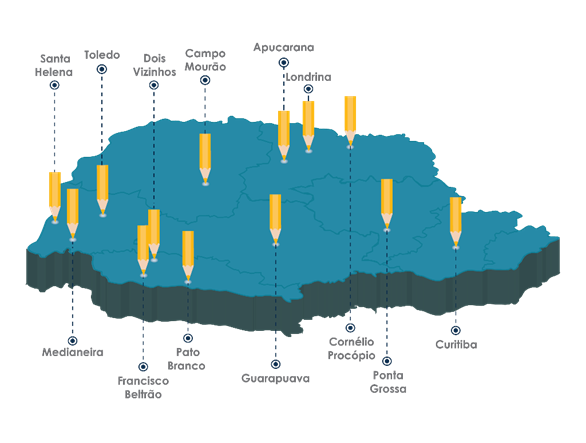
\includegraphics[width=0.7\textwidth]{Caps/Figs/campus_utfpr.png}
        \fonte{\utf}
        \label{fig:13campi}
    \end{figure}
    
    \begin{quadro}
        \centering
        \caption[Diferentes denominações da UTFPR]{As diferentes denominações da UTFPR ao longo de sua existência}        
        \label{qua:denomi}
		\begin{tabularx}{0.7\textwidth}{c >{\centering\arraybackslash}X}
			\toprule%
			\rowcolor{white}\bfseries Ano & \bfseries Denominação\\
			\midrule
			\csvreader[	head to column names,
						late after line=\csvifoddrow{\\}{\\\rowcolor{gray!10}}, 
						separator=pipe]%
						{Caps/Quadros/denominacoesUtfpr.csv}{}%
						{\ano & \denominacao}%
			\bottomrule
			\end{tabularx}
    \end{quadro}

\section{HISTÓRICO DO CÂMPUS}

O município de Toledo está situado na região Oeste do Paraná à 555 km de Curitiba e à 1445 km de Brasília. Pela sua localização geográfica, constitui uma área geopolítica estratégica e de relevância para a integração dos povos do Cone Sul da América. A cidade de Toledo possui aproximadamente 144 mil habitantes, conforme estimativa do Instituto Brasileiro de Geografia e Estatística (IBGE) \cite{ibge2020}.

\nomenclature[A]{IBGE}{Instituto Brasileiro de Geografia e Estatistica}

O município de Toledo é polo microrregional, sede da 18\textordfeminine{} Região Administrativa do Estado do Paraná, congregando 21 municípios que juntos totalizam mais de 350.000 habitantes. O desenvolvimento econômico do município tem atraído crescente número de jovens que buscam oportunidades de trabalho, de estudo e desenvolvimento cultural.

Em face ao projeto de expansão da rede pública federal de ensino, em 2006, a Prefeitura Municipal de Toledo, em conjunto com a Fundação Educacional de Toledo (FUNET) e com o apoio de parlamentares da região protocolou junto ao Governo Federal a solicitação de implantação do Campus Toledo. No mesmo ano realizou-se o exame de seleção para o curso Técnico Integrado em Gastronomia.

\nomenclature[A]{FUNET}{Fundação Educacional de Toledo}

Em 8 de janeiro de 2007 o campus Toledo deu início às suas atividades, sendo oficialmente inaugurado no dia 5 de fevereiro de 2007. Em 12 de fevereiro de 2007 iniciaram-se as aulas do curso Técnico Integrado em Gastronomia. Em agosto do mesmo ano, iniciaram-se as aulas do curso superior de Tecnologia em Processos Químicos no período noturno.

Em 2009 o curso Técnico Integrado em Gastronomia deu lugar ao Curso Técnico Integrado em Informática, o mesmo ano em que o curso superior de Engenharia Industrial Elétrica com ênfase em Automação iniciou suas atividades.

Em 2010 foi vez dos cursos de Engenharia Civil e Licenciatura em Matemática iniciarem suas atividades. Entretanto, nesse mesmo ano, em função das políticas internas da UTFPR, o curso Técnico Integrado em Informática teve sua última entrada de discentes.

Em 2013 o curso Técnico Integrado em Informática formou sua última turma e cedeu lugar para o curso superior de Tecnologia em Sistemas para Internet, o qual iniciou suas atividades no primeiro semestre de 2014. Ainda em 2014 o câmpus Toledo foi contemplado com a autorização para implantação de dois novos cursos de graduação. Assim, os cursos de Engenharia da Computação e Engenharia Bioprocessos e Biotecnologia iniciaram as suas atividades no primeiro semestre de 2015. Nesse mesmo ano foi aberto também o curso de pós-graduação em nível de mestrado acadêmico em Processos Químicos e Biotecnológicos. No ano de 2017, o campus Toledo obteve aprovação para abertura do curso de pós-graduação em nível de mestrado profissional em Matemática com ingresso de alunos previsto para início de 2018. Em 2019, também foi aprovado o Programa de Pós-Graduação em Tecnologias em Biociências (PPGBio) em nível de mestrado profissional.

\nomenclature[A]{PPGBio}{Programa de Pós-Graduação em Tecnologias em Biociências}

\section{HISTÓRICO DO DEPARTAMENTO E/OU DO CURSO}

O curso de graduação em Engenharia Eletrônica no campus Toledo teve o seu funcionamento aprovado pela Resolução N\textordmasculine{} 76/08 – COEPP de 15/08/2008. Iniciou suas atividades em 2009, localizado na Fundação Educacional de Toledo – FUNET, ainda com a denominação de curso de Engenharia Industrial Elétrica com Ênfase em Automação, buscando atender às necessidades da região de qualificação de profissionais atuantes no setor eletroeletrônico e de automação.

\nomenclature[A]{COEPP}{Conselho de Ensino Pesquisa e Pós-graduação da UTFPR}

Em julho 2009 o Ministério da Educação (MEC) publicou um novo catálogo de cursos, em que todas as Engenharias relacionadas a Elétrica deveriam se enquadrar em uma destas cinco categorias: elétrica, eletrônica, controle e automação, telecomunicações e computação. Em função deste catálogo, o colegiado do curso da época decidiu optar por Engenharia Eletrônica. Então, a partir do primeiro semestre de 2010, com mudanças efetuadas na matriz curricular para se enquadrar ao novo catálogo, o curso passou a ser ofertado à comunidade como Engenharia Eletrônica.

\nomenclature[A]{MEC}{Ministério da Educação}

No período de 2010 à 2011 ocorreu a construção e entrega dos Blocos A e C do campus Toledo e o curso foi transferido da FUNET para o campus. As salas de aula e laboratórios do curso foram instalados no Bloco A.

Em meados de 2012, o curso foi submetido ao processo de reconhecimento pelo MEC, obtendo conceito 4.

No ano de 2013, o quadro de professores em regime de dedicação exclusiva totalizava 12 profissionais e ocorreu a formatura da primeira turma do curso de graduação em Engenharia Eletrônica.

\subsection{Primeira atualização na matriz curricular}

Com cinco anos e meio de funcionamento, os professores do curso observaram que alguns ajustes na matriz curricular poderia melhorar  o desempenho dos discentes. Além disso, a alteração também foi motivada pela sinalização do Conselho Regional de Engenharia e Agronomia do Paraná (CREA-PR) que iria atualizar os critérios para concessão do artigo 8\textordmasculine{} da Resolução CONFEA 218/1973 (atribuição na modalidade de eletrotécnica) para os engenheiros recém formados. Até então, os alunos estavam recebendo essa atribuição, mas com as mudanças propostas pelo CREA-PR os novos alunos formados poderiam não obter o artigo 8\textordmasculine{}. Como a região Oeste do Paraná tem uma demanda considerável por Engenheiros Eletricistas, decidiu-se assegurar a aos discentes a garantia da atribuição na modalidade de eletrotécnica. Sendo assim, em 2015, o Núcleo Docente Estruturante (NDE) do curso iniciou discussões para alteração da matriz curricular. Ao final, foi redigido um documento com as modificações propostas que foi aprovado pelo Colegiado do curso e pelo Conselho de Graduações e Educação Profissional da UTFPR (COGEP) por meio da Resolução n\textordmasculine{} 067/15. De forma resumida as modificações aprovadas foram as seguintes:

\nomenclature[A]{CREA-PR}{Conselho Regional de Engenharia e Agronomia do Paraná}
\nomenclature[A]{CONFEA}{Conselho Federal de Engenharia e Agronomia}
\nomenclature[A]{NDE}{Núcleo Docente Estruturante}
\nomenclature[A]{COGEP}{Conselho de Graduações e Educação Profissional da UTFPR}

\begin{itemize}
	\item Deslocamento da disciplina de Física 3 do 2\textordmasculine{} período para o 3\textordmasculine{}  e alteração do pré-requisito;
	
	\item Deslocamento da disciplina de Física 4 do 3\textordmasculine{} período para o 5\textordmasculine{};
	
	\item Deslocamento da disciplina de Probabilidade e Estatística do 5\textordmasculine{} período para o 2\textordmasculine{} e alteração do pré-requisito;
	
	\item Substituição da disciplina de Fundamentos de Programação 2 (60 h) por Fundamentos de Programação Orientada à Objetos (60 h);
	
	\item Substituição da disciplina obrigatória de Instalações Industriais (90 h) pela optativa de Instalações Elétricas Industriais (60 h);
	
	\item Redução da carga horária das optativas de 300 horas para 180 horas;
	
	\item Substituição da disciplina de Fundamentos de Engenharia de Segurança do Trabalho (45 h) para a disciplina de Introdução à Engenharia de Segurança do Trabalho (30 h);
	
	\item Substituição da disciplina de Princípios de Comunicação (75 h) para a disciplina de Fundamentos de Sistemas de Comunicação (60 h);
	
	\item Substituição da disciplina de Circuitos Elétricos 3 (60 h) por Medidas e Sensores (45 h);
	
	\item Deslocamento da disciplina de Materiais e Equipamentos Elétricos do 3\textordmasculine{} período para o 5\textordmasculine{};
	
	\item Mudança da disciplina de Economia do 7\textordmasculine{} período para o 8\textordmasculine{};
	
	\item Alteração do pré-requisito da disciplina de Circuitos Elétricos 1 de Física 3 para Cálculo Diferencial e Integral;
	
	\item Substituição da disciplina de Instalações Prediais (90 h) por Instalações Elétricas Prediais (60 h);
	
	\item Substituir Máquinas Elétricas 1 (60 h) e Máquinas Elétricas 2 (60 h) pela disciplina de Conversão de Energia 1 (60 h);
	
	\item Substituir Máquinas Elétricas 3 (60 h) e Acionamentos Eletromagnéticos (60 h) pela disciplina de Máquinas e Acionamentos (60 h);
	
	\item Criação da disciplina optativa com o nome de Geração, Transmissão e Distribuição de Energia Elétrica (60 h) - alteração visa atender a carga horária mínima para obtenção do artigo 8\textordmasculine{} da Resolução CONFEA 218/1973 (atribuição na modalidade de eletrotécnica);
	
	\item Substituição da disciplina optativa de Sistemas de Potência 1 (75 h) pela optativa de Sistemas de Potência (60 h);
	
	\item Alteração do nome da disciplina de Fundamentos de Programação 1 (60 h) para Fundamentos de Programação (60 h);
	
	\item Deslocamento da disciplina de Metodologia de Pesquisa do 2\textordmasculine{} período para o 8\textordmasculine{};
	
	\item O pré-requisito do Trabalho de Conclusão de Curso 1 foi alterado para: Metodologia de Pesquisa e ter cursado o 7\textordmasculine{} período.
	
	
\end{itemize}

A nova matriz começou a vigorar em 2016 para todos os alunos.

\subsection{Segunda atualização na matriz curricular}

No primeiro semestre de 2018, o NDE do curso propôs a inclusão da disciplina de Eletrônica Analógica 1 como pré-requisito de Medidas e Sensores. Para desenvolver os conteúdos da ementa da disciplina de Medidas e Sensores é necessário um conhecimento básico sobre dispositivos semicondutores (diodos e transistores) – conteúdo abordados em Eletrônica Analógica 1. Sem o pré-requisito proposto seria necessário realizar uma atividade de nivelamento para poder introduzir alguns tópicos da ementa para alunos que ainda não haviam cursado Eletrônica Analógica 1. Por isso, o Colegiado do Curso resolveu aprovar a alteração proposta e enviá-la para apreciação pelo COGEP. Em 04 de junho de 2018 foi publicada a Resolução nº 36/2018 aprovando a alteração, a qual começou a vigorar a partir do segundo semestre de 2018. Maiores detalhes sobre essa alteração podem ser obtidos acessando ao processo SEI 23064.014304/2018-42.

\subsection{Terceira atualização na matriz curricular}

No segundo semestre de 2018, o NDE do curso propôs mais algumas alterações. Foi identificado que a disciplina de Comunicação Oral e Escrita poderia ser alterada para a disciplina de Comunicação Linguística, adotada pelos outros cursos do campus. Dessa forma haveria uma compatibilização das disciplinas entre cursos, maior flexibilização curricular para o aluno. Adicionalmente, a ementa de Comunicação Linguística está atualizada e dentro da formação pretendida. 

A disciplina de Cálculo Diferencial e Integral 3 no curso de Engenharia Eletrônica também tem ementa que não era compatível integralmente com os outros cursos de engenharia do campus. Por isso, resolveu-se adotar a ementa já utilizada nos cursos de Engenharia da Computação e Engenharia Civil. A única mudança foi na ementa da disciplina. Comparando o texto da ementa antiga com o texto da atual o conteúdo ``Funções de variável complexa'' foi excluído. O NDE considerou que esta exclusão não acarretaria problemas ao curso ao na formação dos alunos.

O NDE identificou disciplinas que normalmente apresentam altos índices de reprovação. Estas, poderiam ser divididas em duas, separando a parte teórica da prática. Com essa divisão o discente reprovado na parte teórica e aprovado na parte prática deixaria de consumir recursos do laboratório. Ademais, nas disciplinas iniciais a parte laboratorial fica bastante simples para o aluno reprovado, principalmente quando ele deixa para fazer a disciplina depois que já progrediu razoavelmente na matriz do curso. Dessa forma, o NDE propôs substituir a disciplina de Química, do segundo período, pelas disciplinas de ``Química Básica Teórica'' e ``Química Básica Experimental'' e substituir a disciplina de ``Circuitos Elétricos 1'' para ``Análise de Circuitos Elétricos 1'' e ``Laboratório de Circuitos Elétricos 1''.

O NDE também analisou a retirada de pré-requisito de 3 disciplinas: Probabilidade e Estatística, Empreendedorismo e Gestão de Projetos, aprovando a demanda.

\section{CONTEXTUALIZAÇÃO NACIONAL, REGIONAL E LOCAL}

O Engenheiro Eletrônico é um profissional extremamente flexível e imprescindível em muitos segmentos da economia, com atuação nas mais diferentes áreas da indústria, comércio especializado e serviço.

Nestes últimos anos, aconteceram muitas mudanças no cenário mundial; mudanças políticas, sociais e econômicas. Dessa forma, o estado do Paraná modificou sua política de desenvolvimento, saindo da atividade econômica voltada para a agricultura e pecuária, indo ao encontro da industrialização e consequente modernização de sua economia.

As novas tecnologias, com destaque para a eletrônica, estabeleceram uma nova organização e estrutura para a produção, do que decorre a necessidade de refletir e direcionar esforços para a formação de profissionais para o processo produtivo. Este novo cenário requer profissionais que possuam competências para projetar, executar e manter produtos e serviços que dinamizam o referido processo.

Dessa forma, a oferta do Curso de Engenharia Eletrônica, justifica-se pelos fatores elencados a seguir:

\begin{enumerate}
	
	\item O fato de a UTFPR consolidar-se cada vez mais como uma agência formadora de recursos humanos na área tecnológica;
	
	%\item Adequação do curso de Engenharia Elétrica, Ênfase em Automação, devido a recomendação do MEC para as Engenharias \pdfmarkupcomment{(MEC, 2009)}{não encontrei este documento}, às necessidades regionais;
	\item Adequação do curso de Engenharia Elétrica, Ênfase em Automação, atendendo às necessidades regionais;
	
	\item A oferta de um curso de engenharia visa contribuir com uma preocupação crescente: a carência de profissionais da área de engenharia eletrônica no Brasil;
	
	\item A região Oeste do Paraná possui potencial industrial comprovado, contando com parques industriais estruturados e indústrias nas áreas: alimentos, medicamentos, têxteis e metal mecânica. Além do potencial industrial, a região tem elevada produção agrícola, sendo seus expoentes a suinocultura, avicultura, produção de grãos e leitaria, o que possibilita que inúmeros dispositivos para automação e recursos informatizados possam ser projetados e disponibilizados visando a gestão mais eficiente destas produções.
	
\end{enumerate}

 % CONTEXTUALIZAÇÃO DA INSTITUIÇÃO
    \chapter{VALORES E PRINCÍPIOS INSTITUCIONAIS}

Conforme definido em seu Plano de Desenvolvimento Institucional (PDI), para o quadriênio 2018-2022 \cite{pdiutfpr}, a UTFPR apresenta como valores e princípios institucionais a sua missão, a sua visão e seus valores fundamentais descritos a seguir:

\nomenclature[A]{PDI}{Plano de Desenvolvimento Institucional}

\begin{itemize}[label={}]
	\item \textbf{Missão}: Desenvolver a educação tecnológica de excelência por meio do ensino, pesquisa e extensão, interagindo de forma ética, sustentável, produtiva e inovadora com a comunidade para o avanço do conhecimento e da sociedade;
	
	\item \textbf{Visão}: Ser modelo educacional de desenvolvimento social e referência na área tecnológica;
	
	\item \textbf{Valores fundamentais}:
	
	\begin{enumerate}
		\item Ética: gerar e manter a credibilidade junto à sociedade;
		
		\item Desenvolvimento Humano: formar o cidadão integrado no contexto social;
		\item Integração Social: realizar ações interativas com a sociedade para o desenvolvimento social e tecnológico;
		\item Inovação: efetuar a mudança por meio da postura empreendedor;
		\item Qualidade e Excelência: promover a melhoria contínua dos serviços oferecidos para a satisfação da sociedade;
		\item Sustentabilidade: assegurar que todas as ações se observem sustentáveis nas dimensões sociais, ambientais e econômicas.
		
	\end{enumerate}

\end{itemize}

\section{VALORES/PRINCÍPIOS ORIENTADORES DA GRADUAÇÃO}

A partir da sua missão e visão, a UTFPR estabeleceu a ética, o desenvolvimento humano, a integração social, a inovação, a qualidade e excelência e a sustentabilidade, como os valores fundamentais para a constituição dos princípios e da identidade das graduações.

Os cursos de graduação da UTFPR oferecem formação de recursos humanos para os diversos setores da sociedade, notadamente, os setores da economia envolvidos com práticas tecnológicas e os setores educacionais, a partir da vivência dos estudantes com os problemas reais da sociedade, em especial, àqueles relacionados ao desenvolvimento socioeconômico local e regional, às competências de padrão internacional, ao desenvolvimento e aplicação da tecnologia, e à busca de alternativas inovadoras para a resolução de problemas técnicos e sociais (\href{https://sei.utfpr.edu.br/sei/publicacoes/controlador_publicacoes.php?acao=publicacao_visualizar&id_documento=2803898&id_orgao_publicacao=0}{Resolução COGEP/UTFPR 142/2022, art. 3\textordmasculine}) \nocite{cogep142}.

Para a UTFPR, a formação de seus egressos passa pela sua capacidade de oferecer currículos flexíveis, de articular-se com a sociedade, de estimular a mobilidade acadêmica, de formar para sustentabilidade e interculturalidade, de provocar-se para a inovação curricular e metodológica e de uma forte busca pela internacionalização (\href{https://cloud.utfpr.edu.br/index.php/s/15P0OcMLMdt9Rv7}{PDI 2018-2022}, item 3.4\nocite{pdiutfpr}). A inserção efetiva desses princípios orientadores na dinâmica interna dos cursos de graduação, de torná-los efetivos em sala de aula, nos estudos, na produção científica, no planejamento, na formação continuada, ou seja, em todos os espaços em que atua, é responsabilidade de todos seus atores, e como isso se dará se consolida ao longo desse Projeto Pedagógico de Curso (PPC).

\nomenclature[A]{PPC}{Projeto Pedagógico de Curso}

Fica evidente nas seções 3 a 3.4 do \href{https://cloud.utfpr.edu.br/index.php/s/15P0OcMLMdt9Rv7}{PDI}, como as políticas de ensino serão operacionalizadas a partir da articulação dos valores e princípios institucionais com a formação em inovação, qualidade e excelência; para ética e sustentabilidade; em desenvolvimento humano e em integração social.

\subsection{Valores UTFPR: inovação e qualidade e excelência}

A formação em inovação, qualidade e excelência reportam à busca por mudanças envolvendo postura empreendedora e pela melhoria contínua dos serviços oferecidos para a satisfação da sociedade, conforme \href{https://cloud.utfpr.edu.br/index.php/s/15P0OcMLMdt9Rv7}{PDI 2018-2022} \cite{pdiutfpr}.

Nesse sentido, as atividades de formação envolvem permanentemente a inovação: a curricular e metodológica, no processo didático-pedagógico; no entendimento da tecnologia enquanto conjunto de conhecimentos que conduzem à inovação e contribuem para o desenvolvimento científico, econômico e social; promovendo discussões acerca do papel de cada um na construção de uma forte política de inovação na universidade.

Com intensa interação junto à inovação, a área de empreendedorismo é amplamente difundida e desenvolvida na graduação por meio de mecanismos de suporte para despertar nos estudantes, egressos e servidores da UTFPR o interesse pela área. Os mecanismos institucionais de apoio compreendem a implantação em cada um dos campi da universidade: hotel tecnológico, que viabiliza a pré-incubação para desenvolvimento de projetos e ideias com ênfase em tecnologia e inovação; incubadora de inovações tecnológicas, que viabiliza a incubação de empresas de base tecnológica da comunidade interna ou externa; Empresas Júniores, constituídas por acadêmicos das áreas de formação da UTFPR; e o Programa de Empreendedorismo e Inovação (PROEM).  De forma mais ampla, através do PROEM, professores, pesquisadores, estudantes e ex-alunos empreendedores da Instituição são motivados a desenvolver suas boas ideias a partir da estrutura e do ambiente privilegiando o surgimento de negócios e empresas no âmbito da própria Universidade.  Isto permite ao discente adquirir uma visão mercadológica e da sociedade suficiente para a tomada de atitudes empreendedoras, a capacidade de identificar e gerenciar riscos, capacidade de tomadas de decisão, capacidade de negociar, entre outras habilidades que complementam a formação do Engenheiro Empreendedor.

\nomenclature[A]{PROEM}{Programa de Empreendedorismo e Inovação}

Quanto às inovações curriculares, o curso acompanha as transformações do mundo moderno fomentando novas formas de organização do seu currículo, com abertura ao permanente processo de reexame visando a flexibilização, a compatibilização de conteúdo, a inovação, a sustentabilidade, a interdisciplinaridade e o empreendedorismo.  As inovações curriculares propostas possibilitam o ensino presencial, semipresencial e não presencial aos cursos de graduação (Resolução COGEP n\textordmasculine 142/2022, de 25 de fevereiro de 2022 \cite{cogep142}), incluem o conceito de complemento da carga horária (CCH) que compreendem atividades desenvolvidas fora da sala de aula (\pdfmarkupcomment{Resolução COGEP no 053/2013}{não encontrei essa resolução}), permitem projetos interdisciplinares que tendem a proporcionar a visão do todo e a motivação dos discentes em função de aplicações mais significativas dos conhecimentos adquiridos, permitem avanços tecnológicos pelo emprego de tecnologias de informação e comunicação (TIC) e, por fim, pela criação de diretrizes específicas para cada tipo de curso de graduação permitem a consolidação da identidade e da organicidade no contexto de uma universidade multi campi.

\nomenclature[A]{CCH}{Complemento da carga horária}
\nomenclature[A]{TIC}{Tecnologias de informação e comunicação}

No âmbito do curso há disciplinas vinculadas à inovação, qualidade e excelência integrando a matriz curricular, destacando-se as disciplinas de Economia, Gestão de Projetos e Empreendedorismo. No transcorrer do curso os acadêmicos podem manter contato com a área de inovação por meio de projetos desenvolvidos na disciplina optativa \textit{Enginnering Design Process} em conjunto com empresas com a Metodologia de Ensino Inovador da UTFPR (MEI-U), fundamentando o desenvolvimento inovador do discente. O curso preza pelo reconhecimento das melhores práticas universitárias, pautadas em aliar teoria em prática na formação do Engenheiro.  O curso possibilita o desenvolvimento de habilidade na área eletrotécnica ao criar uma trilha de disciplinas específicas para este fim atendendo a uma demanda de mão de obra local e regional. Dispondo de disciplinas com uma carga horária adequada destinada a práticas e ao desenvolvimento de projetos tendo a disposição laboratórios de ensino modernos e instrumentos. A sinergia com o mercado de trabalho está presente com ações de extensão, estágio em empresas que contribuem para a atualização tecnológica consolidando no âmbito regional como um curso público de excelência.

\nomenclature[A]{MEI-U}{Metodologia de Ensino Inovador da UTFPR}

\subsection{Valores UTFPR: ética e a sustentabilidade}

A formação para a ética está vinculada à formação integral do cidadão, desenvolve o sujeito comprometido seja no seu comportamento, na interação com o outro, ou na geração e manutenção da credibilidade junto à sociedade conforme PPI de 2018 \cite{ppiutfpr}.  A UTFPR é orientada pela ética e pela qualidade de vida de seus servidores e estudantes, prevalecendo um ambiente que visa: ao fortalecimento das relações com todos os envolvidos no desenvolvimento das atividades; à consolidação da imagem institucional e suas ações; e à melhoria contínua nos resultados institucionais.

O fortalecimento do trabalho cooperativo entre as diversas instâncias institucionais, em torno de objetivos comuns, é um direcionamento historicamente construído. O resultado do trabalho em rede permite compartilhar objetivos e procedimentos para a construção de vínculos de interdependência e de complementaridade, possibilitando que as ações realizadas e os resultados obtidos possam ir além dos limites de cada campus, alcançando e fortalecendo a Instituição em prol de suas comunidades.

Cada vez mais o engenheiro deve possuir consciência dos códigos de prática e ética que regem a sua profissão. Sendo assim, os projetos e soluções apresentadas pelos alunos do curso devem considerar esses dois aspectos como elementos norteadores das suas decisões. Especificamente, a Ética Profissional exige que se pense o ensino da Engenharia dentro de um quadro social, ultrapassando os métodos tradicionais de ensino, contextualizando o trabalho nos reflexos que a ciência e a tecnologia causam na sociedade e, mais diretamente, no papel dos que são diretamente responsáveis por introduzi-los no cotidiano de nossas vidas.  Destaca-se a importância de desenvolver nos futuros egressos, herdeiros dessa capacidade de criar a tecnologia que muda o mundo, a possibilidade de viver com um sentido maior de responsabilidade, como nos aponta \citeauthoronline{boff2017} (2017): \pdfmarkupcomment{``nessa urgência de uma visão de valores básicos para proporcionar um fundamento ético à emergente comunidade mundial''}{Verificar se a referência está certa}.

Associada à ética, a sustentabilidade é assegurada nas ações envolvendo as dimensões sociais, ambientais e econômicas. Como importante princípio, o entendimento de sustentabilidade envolve a manutenção do capital natural em sua capacidade de regeneração, reprodução e coevolução, coadunado ao conceito ampliado e integrador de \citeauthoronline{boff2017} (2017), para quem o termo sustentabilidade diz respeito a toda ação destinada a manter as condições energéticas, informacionais, físico-químicas que sustentam todos os seres, e tais condições devem servir de critério para avaliar o quanto temos progredido ou não rumo à sustentabilidade e devem igualmente servir de inspiração para realizar a sustentabilidade nos vários campos da atividade humana.

Comprometimento com as questões sociais e ambientais é esperado que o engenheiro seja capaz de avaliar os impactos sociais e ambientais provocados pelo desenvolvimento tecnológico e identificar oportunidades de atuação para o benefício da sociedade e do meio ambiente. O termo Engenharia da Sustentabilidade enfatiza a engenharia como profissão condutora da inovação tecnológica e capaz de conduzir transformações para uma sociedade sustentável. O Engenheiro deve ser capaz de atender às necessidades do presente sem comprometer a possibilidade das novas gerações atenderem às suas próprias necessidades. No caso da formação do Engenheiro Sustentável, pode-se inferir que esse engenheiro necessita possuir conhecimentos científicos, técnicos, de gestão, éticos, legais, culturais e que saiba produzir soluções que integrem esses conhecimentos e que beneficiem o ``bem comum''. 

Por ser um conhecimento transversal a qualquer curso de engenharia, os professores necessitam buscar integrar questões de sustentabilidade em suas disciplinas por meio de estudos de casos e exercícios que estimulem a reflexão do aluno. As questões ambientais necessitam estar inseridas no contexto local.  Apesar do tema da sustentabilidade estar inserido na disciplina Introdução à Engenharia Elétrica e também constar da unidade curricular? de Ciências do Ambiente. Durante a execução do curso, os professores serão instigados a propiciar aos alunos uma visão do Brasil e do mundo bem como os seus problemas e como o profissional de engenharia pode utilizar a sua criatividade e competência técnica para solucionar ou minimizar esses problemas.

\subsection{Valores UTFPR: desenvolvimento humano}

A formação em desenvolvimento humano, segundo o PDI 2018-2022 \cite{pdiutfpr} e o PPI 2018 \cite{ppiutfpr}, envolve a formação do cidadão integrado ao contexto social a partir de melhorias no processo de ensino e aprendizagem, de ações culturais, artísticas, esportivas e de todas as demais que contribuem para a permanência do estudante, para a sua qualidade de vida, o seu bem-estar individual e social e sua formação humana.  Neste sentido, a instituição prove programas: de acesso e permanência dos alunos por meio do Núcleo de Acompanhamento Psicopedagógico e Assistência Estudantil de Toledo (NUAPE-TD); de promoção da igualdade de oportunidades por meio de editais de ampla concorrência; da ampliação do atendimento presencial e a distância, online e offline por meio de TIC, mantendo a qualidade formal ou técnica; da integração entre concepção e execução, entre o pensar e o fazer, entre teoria e o contexto social pela participação em programas e projetos de ensino, de pesquisa, de desenvolvimento, de inovação e de extensão; e o desenvolvimento da consciência crítica da realidade com a  participação em atividades extracurriculares apoiados pela instituição.  Desse modo, não se deve considerar a formação humana e integral apenas como requisito para formar um bom trabalhador, um bom profissional ou um bom empreendedor. A formação integral do cidadão almejada pela UTFPR, envolve o desenvolvimento de um sujeito: autônomo, numa concepção ampliada de cidadania; preocupado com a preservação do ambiente, dos recursos naturais e das formas de vida do planeta; comprometido com ética e com qualidade de vida. Com um mercado competitivo, o engenheiro deve ser capaz de lidar com o estresse, rejeição ou falhas, suportar pressão e resolver conflitos. O engenheiro deve ser capaz também de planejar uma carreira de tal forma a atender aos seus anseios, sonhos profissionais e objetivos pessoais. Espera-se assim, que esse engenheiro encontre satisfação e realização profissional.

\nomenclature[A]{NUAPE-TD}{Núcleo de Acompanhamento Psicopedagógico e Assistência Estudantil de Toledo}

Sobre o desenvolvimento humano em uma região, as teorias de desenvolvimento econômico convencionais colocam como um dos fatores responsáveis pela falta de dinamismo de uma região, a inexistência de recursos humanos devidamente treinados e preparados, com capacidade de geração de novas tecnologias.  Não obstante, uma região possui aspectos dinâmicos e estratégicos de desenvolvimento, estabelecidos por meio da sucessão de mecanismos que induz e mobiliza o crescimento econômico regional. Além dos aspectos físicos e geográficos, as condições locais para gerar conhecimento, inovação ou fortalecer a atração de investimentos deve ser levada em consideração. O município de Toledo é considerado um polo econômico do oeste paranaense onde verifica-se uma evolução econômica e social bastante significativa no decorrer das décadas a partir do início do século XXI. Considerados os aspectos da evolução econômica, o processo de colonização iniciou-se em 1952 tendo foco na extração madeireira e a policultura para auto consumo que evoluiu a partir da década de 70 para um novo modo de produção e de organização pelas cooperativas agropecuárias e a agroindustrialização.  Em 2020, a produção agropecuária de insumos, a indústria de alimentos e a farmacêutica dinamizam a economia local, em que os produtos e serviços são exportados para outras regiões e/ou países. 

Sob essa perspectiva, o Curso de Engenharia Eletrônica da UTFPR Toledo busca atender às demandas locais ao oferecer conhecimento para ser aplicado no setor produtivo e social. Além disso, atrai e absorve múltiplas habilidades ao integrar estudantes de diversas localidades, promovendo expertises, geradas no processo de ensino, pesquisa e extensão. Esse processo ainda permite maior qualificação profissional e induz à inovação, atração de investimentos localmente e na região, que, por sua vez, gera melhor qualidade de vida e produção de riquezas.

\subsection{Valores UTFPR: integração social}

A formação em integração social diz respeito a realização de ações interativas com a sociedade para o desenvolvimento social e tecnológico. De acordo com o PDI 2018 - 2022 \cite{pdiutfpr}, os cursos da UTFPR, nos diferentes níveis e modalidades de ensino, deverão dar ênfase à ampla formação, que proporcione atitudes interativas e que valorize a atualização constante, promovendo estratégias e métodos de intervenção, cooperação, análise e reflexão, construindo um processo colaborativo e investigativo no âmbito da educação tecnológica, na vivência com os problemas reais da sociedade, voltados para o desenvolvimento sustentável, para a aplicação da tecnologia e para a busca de alternativas inovadoras para resolução de problemas.

Desde a sua criação, o curso tem participado sistematicamente de atividades da região, através de diversas pesquisas e trabalhos direcionados ao setor industrial e ao desenvolvimento tecnológico, ocupando posição de destaque e liderança na formação de recursos humanos. É esperado que o engenheiro seja capaz de avaliar os impactos sociais provocados pelo desenvolvimento tecnológico e identificar oportunidades de atuação para o benefício da sociedade. Não se limitam somente às disciplinas como meios para formação, conta-se também com projetos de extensão desenvolvidos no decorrer do curso que podem apresentar diversificados temas englobando como exemplo a sustentabilidade.  Além disso, o desenvolvimento de um projeto independente da área necessita que se coloque em prática a ética, que deve estar presente nas ações permitindo o contato dos estudantes com a mesma.
 % VALORES E PRINCÍPIOS INSTITUCIONAIS
    \chapter{POLÍTICAS DE ENSINO}
\label{chap:politicas}

Na estruturação de seu PDI 2018-2022 \cite{pdiutfpr} a UTFPR estabeleceu como princípios norteadores para as políticas de seus cursos de graduação a flexibilidade curricular, a articulação com a sociedade, a mobilidade acadêmica, a sustentabilidade, a interculturalidade, a inovação curricular e metodológica e a internacionalização.

Somado a isso as Diretrizes Curriculares dos Cursos de Graduação da UTFPR \cite{cogep142} dão centralidade à sustentabilidade, ao empreendedorismo, à superação do currículo segmentado, ampliando assim a flexibilidade curricular e a proposição de cursos de caráter inovador.

Portanto, a elaboração deste Projeto Pedagógico de Curso está pautada na reformulação do Bacharelado em Engenharia Eletrônica da UTFPR, Câmpus Toledo, com base nos documentos institucionais vigentes, PDI \cite{pdiutfpr} e PPI \cite{ppiutfpr}, bem como em consonância com vertentes contemporâneas de educação em Engenharia no Brasil e no mundo.

A reformulação parte das habilidades e atitudes a serem desenvolvidas pelos discentes segundo a construção de competências do curso de Engenharia, compatíveis com os valores e princípios institucionais, com as Diretrizes Curriculares Nacionais para os Cursos de Engenharia – CNE/CES e com os documentos normativos do conselho de classe – CONFEA/CREA.

Para que o perfil profissional do egresso pretendido pelo Curso de Engenharia Eletrônica seja obtido, a instituição, em conjunto com o curso, proporá práticas pedagógicas para a condução do currículo, visando estabelecer as dimensões investigativa e interativa como princípios formativos e condição central da formação profissional e da relação teoria e realidade. As políticas institucionais promovidas pela UTFPR, e adotadas, de forma direta, no Curso de Engenharia Eletrônica são descritas a seguir.

\section{ARTICULAÇÃO ENTRE A TEORIA E A PRÁTICA E INTERDISCIPLINARIDADE}
\label{sec:artc}

Ao longo de toda sua história, a UTFPR sempre teve o compromisso de romper com a dualidade entre teoria e prática, dimensões estas indissociáveis para a educação integral do indivíduo, pois nenhuma atividade humana se realiza sem elaboração mental, sem uma teoria em que se referencie e lhe dê sustentação. Tal princípio educativo não admite a separação entre as funções intelectuais e as técnicas e respalda uma concepção de formação profissional que unifique ciência, tecnologia e trabalho, bem como atividades intelectuais e instrumentais \cite{pdiutfpr}.

A educação em todos os seus níveis e modalidades deve ser encarada como referencial permanente de formação geral, que encerra como objetivo fundamental o desenvolvimento do ser humano pautado por valores éticos, sociais e políticos, de maneira a preservar a sua dignidade e a desenvolver ações junto à sociedade com base nos mesmos valores. Assim, dentro da carga horária de cada disciplina do curso são desenvolvidos os pressupostos teóricos necessários juntamente com as práticas experimentais/laboratoriais/de campo pertinentes ao conteúdo desenvolvido, utilizando-se dos espaços necessários disponíveis na estrutura do campus.

%\pdfmarkupcomment{As disciplinas que preveem atividades práticas de laboratório têm na ordem de no mínimo 25\% (vinte e cinco por cento) de sua carga horária total voltada para este fim, podendo chegar a 50\% (cinquenta por cento), e estas atividades deverão ser explicitadas nos respectivos Planos de Ensino. As aulas práticas são destinadas a turmas de até 22 (vinte e dois) alunos, ocorrendo desdobramento de turmas quando o número de matrículas excederem esse quantitativo. Nesses casos, a carga horária docente e o desenvolvimento das atividades experimentais são contabilizados e realizados em dobro.}{Essa parte precisamos trabalhar. Verificar se é possível fazer isso durante a matrícula. E se teremos professores suficientes para bancar laboratórios replicados.}

De acordo com a filosofia de concepção de curso, com base nos regimentos internos da UTFPR e nas Resoluções do CONFEA/CREA, a prática acompanhará a teoria com carga horária definida para conteúdos profissionalizantes específicos. Adicionalmente, uma determinada carga horária prática também é contemplada nos núcleos de conteúdos básicos e profissionalizantes, buscando, sempre que possível, a mesma carga horária.

Em sendo assim, cada disciplina definida no curso, apresenta cargas horárias semanais definidas entre Aulas Teóricas – AT e Aulas Práticas – AP, desta forma compondo a carga horária total da disciplina. A integração entre teoria e prática fica a cargo do professor que ministrará a unidade curricular a partir de atividades de campo e/ou laboratoriais, simulações, estudos de caso, projetos, dentre outras, conforme sua escolha. Estas atividades serão sistematizadas de acordo com os seguintes pontos balizadores:

\begin{itemize}
    \item Apresentar problemas em situações reais e/ou simuladas visando a aproximação do discente com contextos reais da engenharia;
    \item Motivar o aluno por meio da aplicação prática de conteúdos trabalhados;
    \item Integrar teoria e prática para melhor compreensão e assimilação dos temas de estudo, destacando o caráter indissociável;
    \item Ser instrumento de avaliação do aluno.
\end{itemize}

Além disso, o curso conta com algumas disciplinas que possuem caráter interdisciplinar, uma vez que articula fundamentos técnicos da engenharia eletrônica aliados a gestão de projetos e ao desenvolvimento de habilidades pessoais e interpessoais. Neste processo, todas as competências trabalhadas durante o curso são integradas em períodos específicos. Pode-se citar como disciplinas interdisciplinares: Medidas e sensores, Sistemas embarcados e Controle Supervisório.

A partir do 7º período, o aluno pode realizar estágio curricular obrigatório, conforme estabelece as Diretrizes Curriculares Nacionais \cite{dcneng}. Neste contexto, o estudante é capaz de colocar em prática todo o ensinamento recebido durante seus anos de estudo no curso, sendo acompanhado por um professor orientador e um supervisor responsável pelo estágio na empresa que o oferece.

Cabe salientar que, o Estágio Curricular Supervisionado deve fornecer condições suficientes para que o aluno possa, de acordo com o PDI, inserir-se com maior facilidade no mercado de trabalho. O PDI destaca: “o estágio curricular é obrigatório para todos os cursos de nível técnico e de graduação, visa à complementação do processo ensino-aprendizagem e tem como objetivos: (i) facilitar a futura inserção do estudante no mundo de trabalho; e (ii) facilitar a adaptação social e psicológica do estudante à futura atividade profissional” \cite{pdiutfpr}.

Adicionalmente, considera-se que o estágio merece destaque por se constituir como espaço privilegiado de aprendizagem, que permite ao estudante integrar-se ao mundo do trabalho, deparando-se com situações, relacionamentos, técnicas e posturas do ambiente profissional que enriquecem e complementam sua formação acadêmico-profissional e empreendedora.

\section{DESENVOLVIMENTO DE COMPETÊNCIAS PROFISSIONAIS}
\label{sec:desen}

%Entende-se por Competências Profissionais, a possibilidade, para um indivíduo, de mobilizar de maneira interiorizada um conjunto integrado de recursos em vista de resolver uma família de situações-problema \cite{scallon2017}. 

%\pdfmarkupcomment{Completar}{O texto aqui precisa seguir as novas DCNs, o texto do PPC vigente (3.2) segue o disposto na DCN antiga.}

Os cursos de graduação da UTFPR, de acordo com o item 3.3.2 Desenvolvimento de competências profissionais do PDI, propõem o desenvolvimento de competências profissionais, entendidas como:

\begin{citacao}
    {[...]} por sua natureza e suas características, a educação profissional e tecnológica deve contemplar o desenvolvimento de competências gerais e específicas, incluindo fundamentos científicos e humanísticos necessários ao desempenho profissional e à atuação cidadã \cite{pdiutfpr}.
\end{citacao}

Primeiramente é pertinente estabelecer que o conceito de competência assumido se refere “a possibilidade, para um indivíduo, de mobilizar de maneira interiorizada um conjunto integrado de recursos em vista de resolver uma família de situações-problema” \cite{scallon2017}. As competências, sejam gerais ou específicas, são desenvolvidas por meio de processos educativos estabelecidos na organização do ensino no curso, envolvendo:

\begin{itemize}
    \item utilização de métodos diferenciados de ensino e novas formas de organização do trabalho acadêmico, que propiciem o desenvolvimento de capacidades para resolver problemas que integram a vivência e a prática profissional;
    \item incorporação dos saberes dos estudantes às práticas de ensino, como forma de reconhecimento de possibilidades de soluções de problemas, assim como de percursos de aprendizagem;
    \item estímulo à criatividade, à autonomia intelectual e ao empreendedorismo;
    \item valorização das inúmeras relações entre conteúdo e contexto, que se podem estabelecer;
    \item integração de estudos de diferentes campos, como forma de romper com a segmentação e o fracionamento, entendendo que os conhecimentos se inter-relacionam, contrastam-se, complementam-se, ampliam-se e influenciam uns nos outros \cite{pdiutfpr}.
\end{itemize}

As competências profissionais são desenvolvidas pelos discentes em todas as disciplinas do curso, iniciando em nível cognitivo baixo até, ao final, alcançarem o nível cognitivo mais alto. Assim, as competências são desenvolvidas gradativamente em várias unidades curriculares e em momentos distintos no decorrer do curso. 

\section{FLEXIBILIDADE CURRICULAR}
\label{sec:flex}

A flexibilidade curricular considera uma construção de curso baseada na diminuição de pré-requisitos, na oferta de diversos caminhos formativos, de disciplinas optativas e disciplinas eletivas, assim como a facilitação da mobilidade acadêmica.

A flexibilização curricular, assegurada pelo PNE 2014-2024, \href{http://www.planalto.gov.br/ccivil_03/_ato2011-2014/2014/lei/l13005.htm}{Lei n° 13.005/2014} \cite{Lei:13005:2014}, é fundamental para atender a demanda social por profissionais que compreendam as novas relações de produção, de trabalho e suas exigências, a demanda pelo conhecimento articulado a produção do saber e de novas tecnologias, a demanda por formação crítica e de profissionais competentes \cite{pdiutfpr}.

Baseada na indissociabilidade entre ensino, pesquisa e extensão, a flexibilização curricular possibilita, por percursos formativos diferenciados, a formação de profissionais competentes, com domínio de habilidades técnicas e cognitivas, com apropriação científica sólida. Os percursos formativos diferenciados rompem com o enfoque unicamente unidade curricular e sequenciado e permitem aos alunos novas formas de apreensão e integração de conhecimentos. Nessa perspectiva, o estudante pode ampliar os horizontes do conhecimento, é capaz de uma visão crítica que lhe permite extrapolar a aptidão específica de seu campo de atuação profissional.

A flexibilização curricular deve possibilitar ao estudante percursos formativos diferenciados para construção das mesmas competências, permitindo inclusive a participação do estudante nas escolhas desses percursos formativos, de ambientes diferenciados de ensino, proporcionando aos discentes visão crítica que lhe permite extrapolar a aptidão específica de seu campo de atuação profissional, estimulando a aprendizagem permanente, a formação de competências e o domínio de habilidades técnicas e cognitivas desejadas.

%\pdfmarkupcomment{É consensual a constatação de estarem superados os modelos de ensino estruturados sob a ótica de grades curriculares inflexíveis, estanques, caracterizadas pela fragmentação e hierarquização rígida das disciplinas (UNIVERSIDADE, 2013a; UNIVERSIDADE,2007a).}{O Alberto V. sugeriu a remoção dete parágrafo, assim como eu sugiro}

Fica evidente, através do PPI \cite{ppiutfpr} e PDI \cite{pdiutfpr}, que a UTFPR tem o compromisso de garantir estruturas curriculares mais inovadoras e flexíveis, permitindo que o aluno tenha participação no ritmo e na direção do seu curso, utilizando-se da melhor forma os mecanismos que a Universidade oferece em termos de atividades acadêmicas na composição de seu currículo.

Este compromisso institucional atende não somente a \href{http://www.planalto.gov.br/ccivil_03/leis/leis_2001/l10172.htm}{Lei n° 10.172/2001} \cite{Lei:10172:2001} e os Pareceres CNE-CES n° 776/97 \cite{parecer776} e n° 583/01 \cite{parecer583}, mas também tem vistas à internacionalização, com medidas que venham a contribuir na flexibilidade dos currículos. A forma como os pré-requisitos são considerados institucionalmente, e a possibilidade de convalidação de disciplinas em bloco ou por saberes e competências são as principais ações que permitem aos cursos considerar, para integralização do currículo do discente, alternativas pessoais e percursos acadêmicos diferenciados.

A proposta é que se permita que várias atividades acadêmicas, que hoje já são desenvolvidas pelo estudante durante sua permanência na universidade, sejam contabilizados no seu histórico escolar. Neste cenário, o curso apresenta duas modalidades de flexibilização curricular: \textbf{vertical} e \textbf{horizontal}. 

A flexibilização vertical é realizada pela organização das disciplinas ao longo de semestres compreendendo o núcleo de formação específica. Ademais, as disciplinas são preferencialmente alocadas em turnos (manhã e tarde) alternados entre cada semestre. Dessa forma o aluno tem a oportunidade de adiantar uma disciplina do próximo semestre e assim concluir o curso em menos de cinco anos, ou então, um aluno que não obteve a aprovação em uma disciplina, pode cursá-la sem necessidade de deixar de cursar as disciplinas do semestre em que se encontra.

O núcleo específico é composto das disciplinas do núcleo comum, cursadas por todos os discentes do curso e das disciplinas optativas das áreas de aprofundamento escolhida pelo aluno, previstas na matriz curricular. Para as disciplinas optativas das áreas de aprofundamento e o Trabalho de Conclusão de Curso (TCC), foi definido um pré-requisito baseado no período, paralelamente aos pré-requisitos baseados em disciplinas. Ou seja, o aluno estará apto a cursar qualquer uma das disciplinas optativas ou TCC desde que esteja matriculado pelo menos no 7\textordmasculine{} período do curso, ou que possua as disciplinas pré-requisitos estabelecidas. Esses pré-requisitos foram estabelecidos porque são imprescindíveis ao bom rendimento escolar.

\nomenclature[A]{TCC}{Trabalho de Conclusão de Curso}

O núcleo não-específico é composto das disciplinas que não constam da matriz curricular do curso escolhido pelo aluno, mas que constituem seus interesses para complementar sua formação em outras áreas de interface, constituindo, assim, um percurso interdisciplinar. Esse núcleo é baseado em uma opção livre, em que o aluno pode cursar um determinado número de disciplinas fora da sua habilitação, sem aprovação prévia dos colegiados e de uma formação complementar realizada em outros cursos, com autorização dos colegiados ou de um número determinado de disciplinas da própria UTFPR que não constam do currículo do aluno ou que são excedentes nos grupos de sua habilitação. Essa escolha fica a critério do aluno. 

A flexibilização horizontal curricular de núcleo não-específico é realizada na UTFPR por meio da modalidade de enriquecimento curricular prevista no Artigo 28 do Regulamento da organização didático-pedagógica dos cursos de graduação da UTFPR \cite{rodp}. Esse artigo permite que o aluno possa cursar uma disciplina que não pertence ao seu curso. Nesse caso, o aluno fica dispensado da exigência de cumprimento dos pré-requisitos. O discente também tem a liberdade de cursar a disciplina de enriquecimento curricular no seu campus de origem ou em qualquer um dos campi da UTFPR, ou mesmo, em instituições com as quais exista acordo de mobilidade e/ou de dupla diplomação.

A flexibilização horizontal também é implementada por meio de atividades ligadas à projetos de extensão, projetos de iniciação científicas, monitoria de disciplinas, línguas estrangeiras, informática, esportes, artes, e de acordo com o seu perfil pessoal, o estudante poderá complementar a sua formação, além de exercitar as atitudes esperadas incentivando-o a interagir com a sociedade em projetos sociais e acadêmicos.

\section{MOBILIDADE ACADÊMICA E INTERNACIONALIZAÇÃO}
\label{sec:mobi}

A mobilidade acadêmica na instituição está prevista em dois planos: o interno (inter campi) e o externo (interuniversitário nacional e internacional).

O plano externo ocorre por meio de convênios mantidos pela UTFPR com Instituições Nacionais e Internacionais, incluído a dupla diplomação, conforme disposto nos Artigos 7\textordmasculine, 9\textordmasculine, 10\textordmasculine, 11\textordmasculine, 16\textordmasculine, 24\textordmasculine, 27\textordmasculine e 28\textordmasculine, do Regulamento da Organização Didático-Pedagógica dos cursos de Graduação da UTFPR \cite{rodp}.

O Programa de Mobilidade estudantil (PME) foi estruturado no campus Toledo com o propósito de aprimorar as atividades de ensino e pesquisa, propiciando a estudantes, docentes e funcionários da UTFPR a vivência de outras culturas e diferentes formas de aprendizagem.

Neste contexto, o Programa de Mobilidade Estudantil da UTFPR tem como objetivo propiciar a mobilidade acadêmica de estudantes regularmente matriculados em cursos de graduação. Todos os programas de mobilidade são de responsabilidade da DIRINTER – Diretoria de Relações Interinstitucionais.

\nomenclature[A]{PME}{Programa de Mobilidade Estudantil}
\nomenclature[A]{DIRINTER}{Diretoria de Relações Interinstitucionais}

Por mobilidade acadêmica entende-se o processo que possibilita o afastamento temporário ao estudante matriculado em uma Instituição de Ensino Superior (IES) para estudar em outra, prevendo que a conclusão do curso se dê na instituição de origem. Ademais, o PME da UTFPR é regido por regulamento próprio e abrange a Mobilidade Estudantil Nacional (MEN) e a Internacional (MEI).

\nomenclature[A]{IES}{Instituição de Ensino Superior}
\nomenclature[A]{MEN}{Mobilidade Estudantil Nacional}
\nomenclature[A]{MEI}{Mobilidade Estudantil Internacional}

\subsection{MOBILIDADE ESTUDANTIL NACIONAL}

A MEN alcança somente estudantes da UTFPR regularmente matriculados em cursos de graduação e os de Instituições Federais de Ensino Superior brasileiras e/ou de Instituições de Ensino Superior do estado do Paraná. Os critérios de elegibilidade dependem do que for estabelecido em edital, mas, em geral, a exigência é que os alunos já tenham cursado e concluído, no mínimo, vinte por cento da carga horária de integralização do curso de origem, bem como tenham, no máximo, duas reprovações acumuladas nos dois períodos letivos que antecedem o pedido de mobilidade.
 
O MEN tem por objetivo promover o intercâmbio entre estudantes da UTFPR e de Universidades Federais e das Estaduais Paranaenses conveniadas, proporcionando-lhes a possibilidade de ampliar seus conhecimentos através da vivência em outras Instituições de Ensino Superior.

Ressalta-se que a Mobilidade Acadêmica não é transferência de Instituição nem de curso.

\subsection{MOBILIDADE ESTUDANTIL INTERNACIONAL}

O programa de cooperação internacional teve início em 1958 com os Estados Unidos, para a implementação do Centro de Formação de Professores da Comissão Brasileiro-Americana de Educação Industrial  (CBAI). Mais tarde, em 1989, a UTFPR firmou convênio com a Fachhochschule de Munique, na Alemanha.

\nomenclature[A]{CBAI}{Comissão Brasileiro-Americana de Educação Industrial}

Nos últimos anos várias instituições alemãs têm mantido intercâmbio de estudantes, possibilitando que alemães estudem e estagiem no Brasil, do mesmo modo que estudantes brasileiros na Alemanha. Houve um crescimento também da preferência pelas universidades de tecnologia francesas. Hoje, além de Alemanha e França, a UTFPR busca ampliar a cooperação acadêmica com outros países tanto no continente europeu quanto americano e africano.

O curso de Engenharia Eletrônica da UTFPR campus Toledo firmou convênio de Dupla Diplomação com o Instituto Politécnico de Bragança (IPB) de Portugal em 2016, permitindo o intercambio de 2 a 4 discentes do curso por ano através desse convênio. Recentemente, no final de 2017, a UTFPR também firmou convênio com a Université de Technologie de Compiègne (UTC) da França, onde os discentes podem ser selecionados através de Editais.

\nomenclature[A]{IPB}{Instituto Politécnico de Bragança}

\section{ARTICULAÇÃO COM A PESQUISA E PÓS GRADUAÇÃO}
\label{sec:pesq}

A UTFPR entende a Pesquisa, a Iniciação Científica, a Inovação Tecnológica, Artística e Cultural como um conjunto de ações que visam a descoberta de novos conhecimentos, consistindo-se em um dos pilares da atividade acadêmica. Pesquisar implica distanciar-se da reprodução acrítica de práticas tradicionais, requer por em jogo processos reflexivos nos quais a interação social e as atividades metacognitivas se fortalecem. Uma visão da investigação como esta é, portanto, um instrumento potente para orientar e favorecer o avanço da ciência e o desenvolvimento profissional \cite{pizzatoconcepccoes}.

O ensino e a pesquisa de forma indissociável colaboram para viabilizar a relação transformadora entre a universidade e a sociedade. Desenvolver projetos de pesquisas que acolham estudantes em diferentes estágios formativos, apoiados nos grupos de estudos e no uso comum da infraestrutura disponível colabora para tanto. A articulação do ensino com as iniciativas de pesquisa e pós-graduação deve considerar o compromisso da instituição com as principais questões e desafios da sociedade, como elemento importante para dupla conscientização, a saber: a do pesquisador ao aceitarem também como desafio acadêmico a busca de soluções para problemas reais; e da sociedade de um modo geral, e do mundo do trabalho em particular, que poderá se beneficiar dos conhecimentos disponibilizados por iniciativas necessariamente submetidas às exigências decorrentes do ``rigor acadêmico''. Para que esse compromisso institucional seja mais efetivo, torna-se importante o esforço de exteriorizar, por um lado, o seu potencial de geração de novos conhecimentos e, por outro lado, o seu desejo que eles sejam compartilhados e aplicados como meio da promoção do desenvolvimento sustentável da região.

O curso de Engenharia Eletrônica da UTFPR, campus Toledo, tem como uma de suas prioridades as atividades de pesquisa, tanto em relação ao corpo docente quanto ao discente. Em relação aos docentes, a pesquisa qualifica as aulas, atualiza os referenciais pedagógicos adotados em sintonia com as discussões em âmbito nacional e internacional e oferece à sociedade e à própria UTFPR as contribuições específicas destas reflexões. Em relação aos alunos, a pesquisa fomenta a formação do Engenheiro(a)-pesquisador(a), isto é, aquele comprometido com o aprimoramento de seus conhecimentos, com o desenvolvimento de novas metodologias e a proposição de soluções para os problemas da área. A pesquisa também complementa os estudos realizados pelos alunos e colabora no desenvolvimento de sua autonomia intelectual.

O incentivo à investigação científica e desenvolvimento tecnológico, diagnosticar e solucionar problemas, é um dos objetivos do curso. Em conformidade com o caráter de Universidade, o curso visa através da articulação, tanto interna quanto externa, de conhecimentos socialmente relevantes que contribuam para formar o quadro dos futuros Engenheiros(as) que venham desempenhar um diferencial no mercado de trabalho, contribuindo dessa forma com profissionais que desempenhem trabalhos de qualidade.

As principais ações de interface do curso com o âmbito científico são por meio do Programa Institucional de Bolsas de Iniciação Científica (PIBIC) e do Programa de Bolsas de Iniciação em Desenvolvimento Tecnológico e Inovação (PIBITI). Os PIBIC/PIBITI têm como meta a inicialização dos discentes em pesquisas científicas e tecnológicas nas diferentes áreas de conhecimento. O programa é apoiado pelo CNPq, Fundação Araucária e UTFPR com a concessão de bolsas, sendo que os alunos também podem participar como voluntários do Programa de Voluntariado em Iniciação Científica e Tecnológica (PVICT). Esses programas objetivam despertar a vocação técnico-científica, incentivar novos talentos potenciais entre os estudantes e contribuir para a formação de recursos humanos para a pesquisa, estimulando pesquisadores produtivos a envolverem alunos de Graduação em atividades técnico-científicas e artístico-culturais. Adicionalmente, o PIBIC/PIBITI/PVICT proporciona aos bolsistas e voluntários, orientados por pesquisador qualificado, a aprendizagem de técnicas e métodos de pesquisa além de estimular o desenvolvimento do ``pensar científico'' e das criatividades decorrentes das condições criadas pelo confronto direto com os questionamentos inerentes à pesquisa. O crescente aumento de projetos homologados e de alunos com Iniciação Científica (IC) ressalta o comprometimento dos docentes do Curso de Engenharia Eletrônica com uma formação sólida e consistente no âmbito científico. %\pdfmarkupcomment{No período de 2016-2017}{atualizar}, foram homologados, junto à Pró-Reitoria de Pesquisa e Pós-Graduação, 12 (doze) projetos de pesquisas dos docentes do curso de Engenharia Eletrônica. Adicionalmente, \pdfmarkupcomment{o Curso foi contemplado com 10 (dez) bolsas de PIBIC/PIBITI}{atualizar}, fomentadas pelo CNPq, UTFPR e Fundação Araucária. 

Os alunos do Curso de Engenharia Eletrônica podem realizar atividades de pesquisa em diferentes áreas do conhecimento, visto que há quatro Grupos de Pesquisa liderados por docentes do curso cadastrados no Diretório do CNPq e certificados pela Instituição, sendo eles: a) Grupo de Eletrônica Aplicada e Sistemas (GEAS); b) Energia Eolicoelétrica; c) Tecnologia de sistemas em geração, controle e eficiência energética; e d) Grupo de processamento eletrônico de fontes alternativas de energia. Os projetos de pesquisa nos quais os estudantes participam apresentam comprovada qualidade acadêmica, mérito científico e orientação adequada pelos docentes do Curso. A participação dos alunos nesses grupos de pesquisa fornece uma ampliação na formação dos bolsistas/voluntários despertando, assim, a vocação científica e incentivando na preparação para ingressar em Programas de Pós-Graduação.

\nomenclature[A]{PIBIC}{Programa Institucional de Bolsas de Iniciação Científica}

\nomenclature[A]{PIBITI}{Programa de Bolsas de Iniciação em Desenvolvimento Tecnológico e Inovação}

\nomenclature[A]{CNPq}{Conselho Nacional de Desenvolvimento Científico e Tecnológico}

\nomenclature[A]{PVICT}{Programa de Voluntariado em Iniciação Científica e Tecnológica}

\nomenclature[A]{IC}{Iniciação Científica}

\section{ARTICULAÇÃO COM A EXTENSÃO}

A extensão universitária é definida como um processo educativo, cultural e científico que se articula ao ensino e a pesquisa de forma indissociável e institucionalizada, viabilizando a relação transformadora entre Universidade e sociedade. Ela oferece um canal de interlocução entre a sociedade e a Universidade, trazendo as demandas da população e os desafios para o desenvolvimento do país para o centro da pesquisa e deste para a sociedade.

De acordo com o artigo 207 da Constituição Brasileira ``as Universidades gozam de autonomia didático-científica, administrativa e de gestão financeira e patrimonial e obedecerão ao princípio da indissociabilidade entre Ensino, Pesquisa e Extensão''. Sendo assim, ensino, pesquisa e extensão devem ser equivalentes e igualmente tratados por parte das Instituições de Ensino Superior, caso contrário, tais entidades estarão se contrapondo à Constituição.

O Curso de Engenharia Eletrônica do campus Toledo tem como pressuposto básico a integração efetiva da extensão universitária ao ensino e à pesquisa, envolvendo os corpos docente e discente, e sempre levando em consideração o compromisso social da Universidade pública brasileira. Além desta indissociabilidade, outros itens das diretrizes básicas definidas no Plano Nacional de Extensão Universitária são compromissos do Curso de Engenharia Eletrônica do campus Toledo: a busca pela interdisciplinaridade e interprofissionalidade; a identificação das demandas da comunidade e das empresas de modo a trazê-las para dentro da Universidade, visando alavancar pesquisas; a articulação de ações que resultem em impacto na formação dos discentes; o incentivo à troca de saberes entre Universidade e sociedade, através da aplicação de metodologias participativas, visando à democratização do conhecimento e a participação efetiva da comunidade na atuação da Universidade. 

Dentro das atividades do curso, a extensão universitária está inserida em trabalhos de conclusão de curso e nos projetos e programas permanentes de extensão desenvolvidos pelos docentes e demais servidores do curso, sempre visando ao estabelecimento de uma forte relação entre ensino, pesquisa e extensão.

O Resolução nº 69/2018 – COGEP, Regulamento de Registro e de Inclusão das Atividades de Extensão nos Currículos dos Cursos de Graduação da UTFPR \cite{cogep69}, estabelece normas para a acreditação das atividades curriculares de extensão visando a curricularização da extensão. A realização de atividades de extensão é obrigatória para todos os estudantes dos cursos regulares de graduação da UTFPR, em um mínimo de dez por cento da carga horária total do seu curso. 
 % POLÍTICAS DE ENSINO
    \chapter{CONTEXTUALIZAÇÃO}

\section{CONTEXTUALIZAÇÃO NACIONAL, REGIONAL E LOCAL}

%A oferta de cursos de engenharia na UTFPR visa a contribuir com uma preocupação crescente: a carência de bons profissionais da área de engenharia no Brasil. \pdfmarkupcomment{Existem atualmente cerca de 550 mil engenheiros no país, uma razão de seis para cada mil pessoas economicamente ativas, enquanto países como Estados Unidos e Japão têm 25. Quase 50\% dos estudantes de Engenharia no Brasil cursam Engenharia Civil, enquanto em países desenvolvidos há um maior percentual em modalidades ligadas a alta tecnologia. A região Oeste do Paraná possui potencial industrial comprovado, contando com parques industriais estruturados e indústrias nas áreas: alimentos, medicamentos, têxteis, informática e metal mecânica. Além do potencial industrial, a região tem elevada produção agrícola, sendo seus expoentes a suinocultura, avicultura, produção de grãos e leitaria, o que possibilita que inúmeros dispositivos para automação e recursos informatizados possam ser projetados e disponibilizados visando a gestão mais eficiente destas produções.}{É necessário encontrar referências de acordo com o texto norteador}

Os avanços tecnológicos que o Brasil vem testemunhando está alterando significativamente as relações entre as pessoas, o setor privado e o setor público. Neste contexto, os Engenheiros em Eletrônica desempenham um papel de grande importância, catalisando as tecnologias emergentes, levando-as ao encontro das necessidades em diversos setores da economia e da sociedade.


\subsection{O setor do agronegócio}

Um exemplo claro desse importante papel do Engenheiro Eletrônico, ocorre de forma muito forte no setor agroindustrial, onde o estado do Paraná ocupa um lugar de destaque no cenário nacional. A agroindústria do Paraná tem seguido bem de perto as tendências mundiais que apontam para a automatização dos processos de cultivo e colheita na agricultura, consequentemente, produzindo melhorias significativas na produtividade desse setor.

Com grande força agrícola na região oeste do Paraná, o município de Toledo é considerado a ``Capital do Agronegócio do Paraná''. Com seu solo fértil e plano, tornou-se um dos maiores produtores de grãos do estado. Segundo dados de 2021 do IBGE, Toledo possuía 144.601 habitantes \cite{ibge2020}. Seu Índice de Desenvolvimento Humano (IDH) alcançou 0,768 em sua última atualização em 2010. O Produto Interno Bruto (PIB) a preços correntes do município alcançou 6 bilhões de reais em 2019 (cerca de R\$ 44.016,71 per capita). 

\nomenclature[A]{IDH}{Índice de Desenvolvimento Humano}
\nomenclature[A]{IDH}{Índice de Desenvolvimento Humano}

A agricultura de precisão, área do conhecimento que evolui com a participação efetiva de profissionais da área de Eletrônica, tem se utilizado de dispositivos sensores avançados, técnicas de comunicação de dados envolvendo conceitos de Internet das Coisas (IoT) e geoprocessamento, processsamento de imagens, dentre outras tecnologias, para trazer ao mercado soluções tecnológicas que inseridas no setor do agronegócio resulta em maior eficiência e desempenho de processos e produtos. 

Nesse sentido, o curso de Engenharia Eletrônica verificou que egressos evm desenvolvendo tecnologias inovadoras para a setor agrícola, princiapamente na área de processamento de imagens das plantações e monitoramento de grãos.

\subsection{O setor tecnológico}

A UTFPR, com mais de um século de existência, tem se consolidado como uma instituição formadora de recursos humanos na área tecnológica em todo o estado do Paraná. O câmpus da UTFPR na cidade de Toledo foi instalado em 2007, sendo fruto da expansão da UTFPR em direção ao interior por meio do programa de apoio a planos de Reestruturação e Expansão das Universidades Federais (REUNI), tendo também contado com a iniciativa da Prefeitura Municipal de Toledo, da Fundação Educacional de Toledo, além outras autoridades e entidades representativas da região. A carência de profissionais é demonstrada no \autoref{qua:cursoskm}, a qual apresenta os resultados de pesquisas de instituições que oferecem cursos correlatos à Engenharia Eletrônica em um raio de 150 km de Toledo. Foram encontradas apenas três instituições com oferta de cinco cursos, incluindo o presente curso.

\nomenclature[A]{REUNI}{Programa de Apoio a Planos de Reestruturação e Expansão das Universidades Federais}

\begin{quadro}
	\centering\small
	\caption[Cursos de Engenharia eletrônica próximos à Toledo/PR]{Cursos de Engenharia eletrônica próximos à Toledo/PR}
	\begin{tabularx}{\textwidth}{>{\centering\arraybackslash}X >{\centering\arraybackslash}X cc}
		\toprule%
		\rowcolor{white}\bfseries Instituição & \bfseries Nome do Curso & \bfseries Cidade & \bfseries Distância\\
		\midrule
		\csvreader[	head to column names,
					late after line=\csvifoddrow{\\}{\\\rowcolor{gray!10}}, 
					separator=pipe]%
					{Caps/Quadros/cursosProx.csv}{}%
					{\inst & \curso & \cidade & \dist}%
		\bottomrule
	\end{tabularx}
	\label{qua:cursoskm}
\end{quadro}

Neste sentido, o curso de Engenharia Eletrônica vem desempenhando um papel importante ao entregar para a sociedade profissionais especializados, capazes de desenvolverem projetos de engenharia envolvendo tecnologias sempre atualizadas. É notável que diversos egressos estão trabalhando com a confecção de projetos elétricos (residenciais ou industriais), automação residencial e desenvolvimento de sistemas eletrônicos industriais.

\section{CONTEXTUALIZAÇÃO DO CURSO}
\label{sec:const}

\pdfmarkupcomment{Do ponto de vista político, o curso de Engenharia Eletrônica também é fruto da expansão da UTFPR em direção ao interior do Estado do Paraná, através do programa de apoio a planos de Reestruturação e Expansão das Universidades Federais (REUNI)}{Ficou repetido em relação à seçao anterior}. Adicionalmente, o curso contou com a iniciativa da Prefeitura Municipal de Toledo, da Fundação Educacional de Toledo (FUNET) e da UTFPR – Câmpus Medianeira para iniciar as suas atividades. Analisando pelo aspecto econômico, os engenheiros têm papel fundamental para a economia do país, de tal forma que alguns indicadores econômicos se baseiam na atividade de engenharia ou na quantidade de engenheiros formados no país/região. A criação do curso busca atender às necessidades da microrregião de Toledo, mediante formação de profissionais para atuar no setor eletroeletrônico, de automação e de elétrica. \pdfmarkupcomment{A oferta do curso de engenharia eletrônica visa contribuir com uma preocupação crescente: a carência de profissionais da área de engenharia no Brasil. Existem atualmente cerca de 550 mil engenheiros no país, uma razão de seis para cada mil pessoas economicamente ativas, enquanto países como Estados Unidos e Japão têm 25. Quase 50\% dos estudantes de Engenharia no Brasil cursam Engenharia Civil, enquanto em países desenvolvidos há um maior percentual em modalidades ligadas a alta tecnologia, como eletrônica, por exemplo.}{também repette}

\nomenclature[A]{FUNET}{Fundação Educacional de Toledo}

A região Oeste do Paraná possui potencial industrial comprovado, contando com parques industriais estruturados e indústrias nas áreas: alimentos, medicamentos, têxteis, informática e metal mecânica. Além do potencial industrial, a região tem elevada produção agrícola, sendo seus expoentes a suinocultura, avicultura, produção de grãos e leitaria, o que possibilita que inúmeros dispositivos eletrônica para automação e recursos informatizados possam ser projetados e disponibilizados visando a gestão mais eficiente destas produções. Além das evidências regionais, o mercado global e a velocidade dos avanços tecnológicos, principalmente nas áreas de elétrica, eletrônica, automação e computação, têm gerado carência de profissionais qualificados, capazes de atender as demandas e acompanhar tais mudanças. O mercado relacionado à eletrônica é totalmente globalizado, mas com uma forte demanda local, exigindo dos profissionais a apresentação de soluções muitas vezes personalizadas, que demandam menores custos e maior satisfação dos clientes. Adicionalmente, percebe-se o avanço do emprego de dispositivos eletrônicos nas mais diversas áreas, incluindo o agronegócio, processamento de alimentos, indústria química e os outros ramos da engenharia. Desta forma, um profissional que combine um sólido embasamento em sua área de atuação, com forte perfil inovador, e liderança estará melhor adaptado e mais propenso a atender as necessidades locais.

Considerando o cenário futuro, a direção do Câmpus Toledo da UTFPR, com apoio da Reitoria e da Pró-reitoria de Relações Empresariais e Comunitárias (PROREC) firmaram um convênio com o Biopark, um empreendimento privado, sediado em Toledo e que visa se transformar em um parque tecnológico referência em biociências e biotecnologia. A UTFPR recebeu a doação de um terreno com uma área de 37.375 m$^2$ para a instalação de um complexo da Universidade Tecnológica Federal do Paraná (UTFPR). O estabelecimento desse parque tecnológico deve fortalecer ainda mais a região na área de tecnologia, aumentando a demanda por engenheiros. 

\nomenclature[A]{PROREC}{Pró-reitoria de Relações Empresariais e Comunitárias}

A evolução Histórica do curso de Engenharia Eletrônica pode ser resumida como:

\begin{enumerate}
	\item 	Ingresso da primeira turma em 2009 com a denominação de curso de Engenharia Industrial Elétrica com Ênfase em Automação;
	\item 	Mudança do nome do curso para Engenharia Eletrônica no início de 2010;
	\item	Em 2012, ocorreu o reconhecimento do curso pelo MEC, que atribuiu conceito 4 ao curso;
	\item	Em 2013, ocorreu a formatura da primeira turma;
	\item	Em 2017, o curso foi avaliado no ENADE, obtendo conceito 5;
	\item	Em 2019, o curso completou 10 anos de existência e foi submetido a uma nova avaliação do ENADE, obtendo conceito 4.
\end{enumerate}

Com base neste contexto, a UTFPR estruturou seu curso de Engenharia Eletrônica, que oferecerá uma formação ampla e diversificada, dentro da grande área da Elétrica, que inclui as áreas básicas Matemática, Física, Química, Informática e Humanas, que, visam proporcionar melhores condições para as práticas. Também engloba áreas mais aplicadas, as de cunho profissionalizante, tais como Eletrônica Analógica e Digital, Automação e Controle, Processamento Digital de Sinais e Sistemas Embarcados/Microcontrolados.
 
Dessa forma, o egresso do curso de Engenharia Eletrônica pode atuar em diversas áreas, abrangendo indústrias de materiais, dispositivos e instrumentos elétricos, eletrônicos e de informática, escritórios de engenharia, empresas de geração e distribuição de energia, empresas de consultoria e assessoramento, empresas de software, serviços públicos e instituições de ensino e pesquisa, produção industrial, desenvolvimento de software, gestão de pessoas e de processos, desenvolvimento de hardware e software para os processos de automação. Integrado a esse contexto, o curso de Engenharia Eletrônica tem papel fundamental na região, contribuindo para o seu desenvolvimento.

\section{QUADRO DE DADOS GERAIS DO CURSO}

O \autoref{qua:geral} representa os dados gerais do curso.

\begin{quadro}
	\centering\small
	\caption[Dados gerais do curso]{Dados gerais do curso}	
	\label{qua:geral}
	\begin{tabularx}{0.8\textwidth}{|>{\raggedleft\arraybackslash}X || >{\raggedright\arraybackslash}X|}
		\hline
		\csvreader[	head to column names,
					separator=pipe,
					late after line=\csvifoddrow{\\}{\\\rowcolor{gray!10}}, 
					table head=\hline, 
					table foot=\hline]%
					{Caps/Quadros/quadroGeral.csv}{}{%
						\tipo & \dado 
					}
		\hline
	\end{tabularx}
	
\end{quadro}

\section{FORMA DE INGRESSO E VAGAS}

O acesso aos cursos superiores da UTFPR desde o ano de 2009 ocorre de acordo com o Sistema de Seleção Unificado (SISU) que utiliza a nota do Exame Nacional do Ensino Médio (ENEM), conforme a Deliberação n\textordmasculine 04/2009 do Conselho Universitário da UTFPR \cite{sisuutfpr}.

\nomenclature[A]{SISU}{Sistema de Seleção Unificado}
\nomenclature[A]{ENEM}{Exame Nacional do Ensino Médio}

As entradas definidas no parágrafo anterior compreendem 44 vagas semestrais, sendo que os alunos ingressantes iniciam o curso no período vespertino, havendo alternância dos próximos períodos para matutino (períodos pares) e vespertino (períodos ímpares). Tal oferta de vagas é definida em decorrência dos parâmetros do MEC quanto à liberação de vagas docentes no ato da autorização dos cursos e também do planejamento da própria UTFPR em termos das dimensões das salas de aulas teóricas e práticas.

Também são admitidos alunos por meio de editais de processos seletivos para vagas remanescentes ou transferência a partir do segundo semestre, obedecendo às normas aprovadas pelo Conselho de Graduação e Educação Profissional (COGEP) da UTFPR.

\section{OBJETIVOS DO CURSO}
\label{sec:obj}

\pdfmarkupcomment{Em função do planejamento estratégico institucional e das ações definidas pelo planejamento do curso foram definidos os objetivos descritos abaixo:}{RECOMENDA-SE REDUZIR ESSE TEXTO}

\begin{enumerate}
	\item	Formar um profissional generalista, que atua na área de materiais eletroeletrônicos; sistemas de medição e de controle eletroeletrônico; desenvolvimento de sistemas, produtos e equipamentos eletrônicos, sistemas embarcados, conversores de energia e instalações elétricas.
	\item	Formar um profissional que estuda, projeta e especifica materiais, componentes, dispositivos e equipamentos eletroeletrônicos, eletromecânicos, magnéticos, ópticos, de instrumentação, sensores e atuadores de transmissão e recepção de dados, de áudio/vídeo, de segurança patrimonial e de eletrônica embarcada.
	\item	Capacitar o graduado a planejar, projetar, instalar, operar e manter sistemas e instalações eletrônicas, instalações elétricas, equipamentos, sistemas de medição e instrumentação eletroeletrônica, de acionamentos de máquinas elétricas, de controle eletrônico e de automação e de sistemas eletrônicos embarcados.
	\item	Fornecer embasamento teórico para coordenar e supervisionar equipes de trabalho, realizar estudos de viabilidade técnico-econômica, executar e fiscalizar obras e serviços técnicos; e efetuar vistorias, perícias e avaliações, emitindo laudos e pareceres.
	\item	Imbuir no profissional a ética, a segurança, a legislação e os impactos ambientais.
	\item	Fornecer um embasamento sólido que permita ao aluno dar prosseguimento a seus estudos, expandindo sua área de atuação, atuando em áreas multidisciplinares, ou buscando pós-graduação.
	\item	Atender a legislação profissional, habilitando o graduado a atuar em um amplo espectro da Engenharia Elétrica e Eletrônica, com atribuições condizentes com as resoluções relativas a atribuições profissionais do Conselho Federal de Engenharia e Agronomia (CONFEA) e do Conselho Regional de Engenharia e Agronomia (CREA).
	\item	Estabelecer-se como um curso flexível permitindo ao aluno participar de programas de mobilidade acadêmica, de intercâmbios e de programas de dupla diplomação.
	\item	Permitir a celebração de convênios de dupla diplomação com universidades estrangeiras.
	\item	Permitir ao egresso do curso a atualização constante através de disciplinas optativas nas áreas de aprofundamento, com a possibilidade de serem cursadas em outros campi da UTFPR, facultando-lhe agregar novas competências e atribuições profissionais junto ao sistema CONFEA/CREA.
\end{enumerate}

Pretende-se que o Curso venha a se distinguir pela acentuada integração com empresas, pela busca de integração com cursos de Pós-Graduação, pela significativa visão sistêmica e integração entre software e hardware, pela integração das disciplinas de Trabalho de Conclusão de Curso (TCC), pela educação continuada, pela possibilidade de convalidação de créditos cursados em Universidades estrangeiras, pelo incentivo ao empreendedorismo, pela diversidade das Áreas de Conhecimento, bem como pela elevada carga horária em laboratórios.

\section{PERFIL DO EGRESSO}
\label{sec:perf}

Além das características estabelecidas no Art. 3\textordmasculine{} das DCNs, o egresso do curso superior de Bacharelado em Engenharia Eletrônica é um profissional versátil capaz de propor soluções em sistemas eletroeletrônicos em contexto local e global, considerando legislação, normas técnicas, preceitos ético-políticos, sustentabilidade, inovações, e bem estar social. Tal profissional se caracteriza por conceber sistemas analógicos, de potência, de processamento digital, de controle automação e eletrotécnica. Poderá atuar em empresas públicas ou privadas de base tecnológica, no desenvolvimento de hardware e software e a sua integração com outros sistemas, bem como na capacitação de equipes de profissionais da área tecnológica. Sendo capaz de:


\renewcommand{\labelenumi}{\roman{enumi}}
\begin{enumerate}
	\item Desenvolver sistemas eletroeletrônicos eficazes, gerenciando os recursos tecnológicos, de forma sustentável; 
	\item Gerenciar o desenvolvimento de projetos, segundo normas e critérios técnicos de segurança e de desempenho, com senso crítico e atitude colaborativa. 
	\item Capacitar equipes de profissionais da área tecnológica, com comunicação qualificada.
\end{enumerate} 

As DCNs \cite{dcneng} estabelecem competências gerais em seu Artigo 4\textordmasculine, indicando também no parágrafo único deste Artigo o estabelecimento de competências específicas, de acordo com a habilitação e a ênfase do curso. Dessa forma, as Competências específicas do curso de Engenharia Eletrônica redigidas pelo NDE são:

\begin{itemize}
	\item \textbf{Eletrônica}: conceber e/ou intervir em sistemas eletrônicos com autonomia, integrando circuitos analógicos, computação embarcada, controle de sistemas e 	processamento digital de informações e considerando uma documentação clara e concisa;
	\item \textbf{Científica}: produzir investigação científica integrando modelos de fenômenos naturais, conhecimentos técnico-científicos, escrita e metodologia científica com honestidade intelectual e senso crítico;
	\item \textbf{Empreendedora}: Analisar ou propor negócios, com responsabilidade compartilhada e atitudes empreendedora e cooperativa, por meio da articulação de informações técnicas e conceituais e avaliação do micro e macroambiente;
	\item \textbf{Eletrotécnica}: Conceber e/ou intervir em sistemas elétricos com autonomia, integrando instalações elétricas , máquinas elétricas e sistemas de potência, considerando uma documentação clara e concisa e segurança elétrica.
\end{itemize}

O desenvolvimento dessas competências, no âmbito do curso de Engenharia Eletrônica, é discutido na \autoref{sec:comp}.
 % CONTEXTUALIZAÇÃO
    \chapter{ORGANIZAÇÃO DIDÁTICO PEDAGÓGICA}
\label{chap:matriz}

O curso Superior de Engenharia Eletrônica do Câmpus Toledo da UTFPR  é estruturado de acordo com: a Lei nº 9.131, de 24 de novembro de 1995 \cite{Lei:9131:1995}; a Lei nº 9.394, de 20 de dezembro de 1996 \cite{Lei:9394:1996}; a Lei nº 11.184, de 7 de outubro de 2005 \cite{Lei:11.184:2005}; o Estatuto e Regimento Geral da UTFPR \cite{estatutoutfpr}; as Diretrizes Curriculares Nacionais do Curso de Graduação em Engenharia \cite{dcneng}; a Resolução n\textordmasculine{} 142/2022 – COGEP/UTFPR, de 25 de fevereiro de 2022 \cite{cogep142}; e às demais diretrizes e regulamentos internos aplicáveis. A concepção de ensino e aprendizagem do curso, a matriz curricular, os procedimentos de avaliação e os instrumentos de apoio expressos no Projeto Pedagógico de Curso (PPC), são construídos coletivamente e submetidos ao Conselho de Graduação e Educação Profissional (COGEP) para aprovação, em modelo e prazo estabelecido.

Segundo o PPI:

\begin{citacao}
	``A  UTFPR  deve  contribuir  para  o  avanço  conceitual  da educação profissional e tecnológica, tomando como princípio a formação integral do homem,  em  bases  científicas  e  ético-políticas,  entendendo  que  o  exercício  das atividades humanas não se restringe ao caráter produtivo, mas compreende todas as dimensões: social, política, cultural e ambiental'' \cite{ppiutfpr}.
\end{citacao}

Dessa forma, a estrutura curricular do Curso de Engenharia Eletrônica da UTFPR – Campus Toledo possui bases na demanda do mercado regional (veja a \autoref{sec:const}), demanda essa tanto de qualificação profissional, como de características socioeconômicas. Para dar atendimento à demanda do mercado de um profissional com um perfil diferenciado, não só em tecnologia, mas também voltado para o desenvolvimento social e sustentabilidade, a organização do Curso de Engenharia Eletrônica apresenta bases científicas e de gestão de nível superior dimensionada e direcionada às terminalidades da formação do engenheiro.

A organização didático pedagógica deste PPC promove as políticas de ensino e de graduação, previstas nos documentos institucionais norteadores PDI \cite{pdiutfpr} e PPI \cite{ppiutfpr}. As políticas de ensino são as elencadas na seção ``3.3 POLÍTICAS DE ENSINO'' do PDI:

\begin{itemize}
	\item Articulação entre a teoria e a prática;
	\item Desenvolvimento de competências profissionais;
	\item Flexibilidade curricular;
	\item Mobilidade acadêmica;
	\item Articulação entre ensino, pesquisa e extensão.
\end{itemize}

Da mesma forma, as políticas de graduação são elencadas na seção ``3.4 POLÍTICAS DE GRADUAÇÃO'' do PDI:

\begin{itemize}
	\item Flexibilidade curricular;
	\item Articulação com a sociedade;
	\item Mobilidade acadêmica;
	\item Sustentabilidade;
	\item Interculturalidade;
	\item Inovação curricular e metodológica;
	\item Internacionalização.
\end{itemize}

O Curso de Engenharia Eletrônica promove a aprendizagem de conhecimentos estruturados vinculados ao desenvolvimento de competências, em uma dinâmica que enfatiza a prática profissional sem excluir as dimensões sociais e ambientais da qual faz parte. As disciplinas, não mais isoladas, são promotoras do saber, saber fazer e saber ser, se responsabilizando pelo currículo vivo formador de profissionais aptos a mobilizar, integrar e aplicar adequadamente esses conhecimentos. A metodologia do curso envolve processos de participação do estudante que permite a constante construção do conhecimento.

Os conceitos são apresentados a partir dos conhecimentos expostos em livros didáticos, artigos científicos, situações reais e outros materiais bibliográficos pertinentes, conduzidos pela experiência dos docentes. Também são incentivados projetos que permitam a análise reflexiva e o aprendizado da prática profissional pelo discente. Procura-se continuamente estabelecer a interdisciplinaridade relacionando os conteúdos das diversas disciplinas que compõem o curso.

A estrutura apresentada, propõe a intencionalidade em trabalhar habilidades e atitudes do futuro engenheiro. O corpo docente, com sua experiência adquirida, permitirá momentos de aprendizagem relacionados ao desenvolvimento dessas habilidades e atitudes através de um projeto de currículo para esse fim.

Neste contexto, esse projeto de estrutura curricular é apresentado em detalhes nas seções posteriores, bem como sua relação com as políticas de ensino e de graduação indicadas no início desta seção.


\section{ORGANIZAÇÃO CURRICULAR}

A matriz curricular do curso de Engenharia Eletrônica da UTFPR é estruturada em dez semestres sob o regime de matrícula por disciplina com entrada anual de 88 acadêmicos. Sua carga horária totaliza \the\value{horasT} h de atividades com conteúdo de natureza profissionalizante, científica, humanística, extensionista e cultural.

A organização da matriz curricular do curso contempla os objetivos de instigar o interesse pela ciência e tecnologia e, ao mesmo tempo, fornece um sólido embasamento para o conteúdo profissionalizante. Isto é alcançado apresentando disciplinas profissionalizantes o mais cedo possível, ao mesmo tempo que o aluno tem uma prévia do que será ministrado adiante no curso através da disciplina de Introdução à Engenharia. A maioria das disciplinas possui carga horária em laboratório, com experimentos realizados nas áreas de física, química e eletrônica desde o primeiro semestre. As disciplinas da área de formação profissionalizante estão presentes a partir do terceiro semestre e são desenvolvidas em sua maior parte em laboratório. Especificamente, os conteúdos de computação são apresentados desde o primeiro semestre, enquanto os conteúdos de engenharia elétrica e eletrônica são apresentados desde o terceiro. Além disso, a sequência de pré-requisitos das disciplinas permite a inclusão de atividades interdisciplinares desde o início do curso.

%As atividades acadêmicas presenciais são divididas em Atividades Teóricas (AT) e Atividades Práticas (AP). As ATs consistem na apresentação de conteúdos teóricos em sala de aula. Já as APs têm vistas ao desenvolvimento prático dos conteúdos, consistindo de experimentos, atividades de laboratório, ou visitas técnicas. 

As atividades acadêmicas são divididas em atividades teóricas (AT) e práticas (AP), conforme Art. 20 das Diretrizes Curriculares dos Cursos de Graduação Regulares da UTFPR \cite{cogep142}. As ATs correspondem às atividades, de caráter presencial ou não, utilizadas para o desenvolvimento e compreensão de conceitos e de teorias. Já as AP têm vistas às atividades, de caráter presencial ou não, utilizadas para o desenvolvimento prático de conteúdos, tais como: atividades de laboratório, desenvolvimento de projetos, estudos de caso, visitas técnicas, levantamentos em campo, produção de textos, dentre outras.

%O Art. 24 em seu parágrafo 1\textordmasculine{} considera que os projetos pedagógicos dos cursos da UTFPR devem dar ênfase a AP. Para cursos de Engenharia, a carga horária de AP deve ser coerente com a formação pretendida. Objetiva-se, com isto, formar um profissional diferenciado, apto a lidar com problemas de ordem prática e pronto para lidar com as necessidades imediatas do mercado de trabalho.

Algumas unidades curriculares também possuem parte da carga horária  em atividades não-presenciais (ANP), que correspondem a processos de ensino e aprendizagem desenvolvidos para além dos tempos e espaços da sala de aula. São mediadas por tecnologias digitais de informação e comunicação, desenvolvidas numa relação dialógica entre docentes e estudantes.

\nomenclature[A]{AT}{Atividades Teóricas}
\nomenclature[A]{AP}{Atividades Práticas}
\nomenclature[A]{ANP}{Atividades não-Presenciais} 

O curso de Engenharia Eletrônica dá ênfase as APs. Objetiva-se, com isto, formar um profissional diferenciado, apto a lidar com problemas de ordem prática e pronto para lidar com as necessidades imediatas do mercado de trabalho.



%A Construção curricular deve responder diretamente aos objetivos formativos. Considerando as metas educacionais para formação profissional percebe-se que para alcança-las os projetos de ensino superior precisam propor mudanças significativas e inovadoras em suas organizações curriculares.

%Assim, é imperativo a construção de currículos inovadores e estrategicamente orientados à aprendizagem significativa, ao desenvolvimento integrado e sustentável, às necessidades, aspirações e expectativas dos alunos e à transformação da realidade em que vivem.

%No início da apresentação da organização curricular deve conter a proposta que fundamenta o curso, pois, são os fundamentos teórico metodológicos que sustentam as decisões sobre a escolha entre uma ou outra matriz curricular. A organização curricular do curso deve apresentar as unidades curriculares agrupadas por áreas de conhecimento, número de períodos, organização de temas transversais, integração horizontal e vertical. Incluir aqui como será desenvolvido no curso o ciclo de humanidades (art. 25 e 26 da Resolução COGEP 90/2018). Descrever se, como e quanto serão utilizados de momentos de aprendizado não presenciais ao longo do curso


\section{MATRIZ CURRICULAR}
\label{sec:matriz}

A matriz curricular do Curso de Engenharia Eletrônica é construída em consonância com os objetivos do curso e da Instituição, atendendo ao perfil do egresso (ver \autoref{sec:perf}), após as discussões dos integrantes do NDE.

Os conteúdos trabalhados devem ter significado aos estudantes, possibilitando uma aprendizagem consistente e significativa. Entende-se que os conhecimentos técnicos não podem estar separados da formação geral e humanística. Os eixos norteadores, destacados, são considerados prioritários e serão desenvolvidos durante toda a trajetória do curso, quais sejam, como Meio ambiente, Ética e Cidadania, Relações Étnico-Raciais, Direitos Humanos, a construção de valores de solidariedade, inclusão, cooperação e respeito à Diversidade.

A partir desta perspectiva, a estruturação curricular do curso seguindo as diretrizes curriculares para os cursos de Engenharia \cite{dcneng}, é embasada em três Núcleos de Conteúdos, com a necessária interligação entre si:

\begin{enumerate}
	\item 	Núcleo de Conteúdos Básicos;
	\item 	Núcleo Conteúdos Profissionalizantes;
	\item 	Núcleo Conteúdos Profissionalizantes Específicos.
\end{enumerate}

Quanto a extensão, os discentes do Curso podem desenvolver em conjunto com a Universidade:

\begin{itemize}
	\item 	Projetos de Educação e Inclusão Social;
	\item	Ações para Desenvolvimento Econômico e Responsabilidade Social;
	\item	Atividades de Valorização da diversidade, do meio ambiente, da memória cultural, da produção artística e de patrimônio cultural;
	\item	Projetos de Educação Ambiental e de Desenvolvimento Nacional Sustentável.
\end{itemize}

% Retirado do PPC de campo mourão
A estrutura curricular tem como base a demanda do mercado regional e nacional, sendo norteada pela qualificação profissional e ao atendimento das necessidades socioeconômicas. Para dar atendimento à demanda do mercado por profissionais com um perfil diferenciado, não só em tecnologias emergentes, como também voltado para o desenvolvimento social, a organização do Curso de Bacharelado em Engenharia Eletrônica apresenta bases científicas e de gestão de nível superior dimensionada e direcionada às terminalidades da formação do engenheiro. %Estruturada em dez semestres sob o regime de matrícula por unidade curricular, sua carga horária totaliza \the\value{horasT} h de atividades com conteúdo de natureza profissionalizante, científica, humanística e cultural.

%A organização da matriz curricular do curso contempla os objetivos de instigar o interesse pela ciência e tecnologia e, ao mesmo tempo fornecer um sólido embasamento para o conteúdo profissionalizante. Isto é alcançado apresentando disciplinas profissionalizantes o mais cedo possível, ao mesmo tempo em que o aluno tem uma prévia do que será ministrado adiante no curso através da disciplina de Introdução à Engenharia. A maioria das disciplinas possui carga horária em laboratório, com experimentos realizados nas áreas de física, química e eletrônica desde o primeiro semestre. As disciplinas da área de formação profissionalizante estão presentes em quase todos os semestres e são desenvolvidas em sua maior parte em laboratório. Além disso, os conteúdos de engenharia elétrica e eletrônica são apresentados desde o primeiro semestre, buscando a motivação do discente desde o início de sua jornada acadêmica.

%As atividades acadêmicas são divididas em atividades teóricas (AT) e práticas (AP), conforme Art. 20 das Diretrizes Curriculares dos Cursos de Graduação Regulares da UTFPR \cite{cogep142}. As ATs correspondem às atividades, de caráter presencial ou não, utilizadas para o desenvolvimento e compreensão de conceitos e de teorias. Já as AP têm vistas às atividades, de caráter presencial ou não, utilizadas para o desenvolvimento prático de conteúdos, tais como: atividades de laboratório, desenvolvimento de projetos, estudos de caso, visitas técnicas, levantamentos em campo, produção de textos, dentre outras.

%O Art. 24 em seu parágrafo 1\textordmasculine{} considera que os projetos pedagógicos dos cursos da UTFPR devem dar ênfase a AP. Para cursos de Engenharia, a carga horária de AP deve ser coerente com a formação pretendida. Objetiva-se, com isto, formar um profissional diferenciado, apto a lidar com problemas de ordem prática e pronto para lidar com as necessidades imediatas do mercado de trabalho.

%Ainda, o curso desenvolve as ações de: (i) popularização científica e tecnológica; (ii) disseminação tecnológica em escolas do ensino médio e fundamental; (iii) ações para integração com o mundo do trabalho e (iv) projetos de educação ambiental e de desenvolvimento regional sustentável.
%% Fim da cópia

O \autoref{qua:matriz} apresenta a matriz curricular do curso de Engenharia Eletrônica do campus Toledo da UTFPR. \pdfmarkupcomment{As unidades curriculares são codificadas por cores, sendo verde claro: obrigatórias do ciclo de humanidades; verde escuro: optativas do ciclo de humanidades; cinza: optativas específicas; e amarelo: demais unidades curriculares}{Verificar como fica a codificação das cores, até o momento não existe uma orientação.} %As seções \ref{sub:reg} à \ref{sub:extch} resumem as informações do referido quadro.

As unidades curriculares do curso, apresentadas na matriz anterior (\autoref{qua:matriz}), apresentam em sua constituição carga horária teórica e prática, com codificação em cada unidade curricular, conforme apresentado na \autoref{fig:legenda}. Portanto, diversas disciplinas promovem a política de ensino ``Articulação entre teoria e prática''.

\begin{figure}[hbt!]
	\centering
	\caption{Codificação das unidades curriculares da Matriz}
	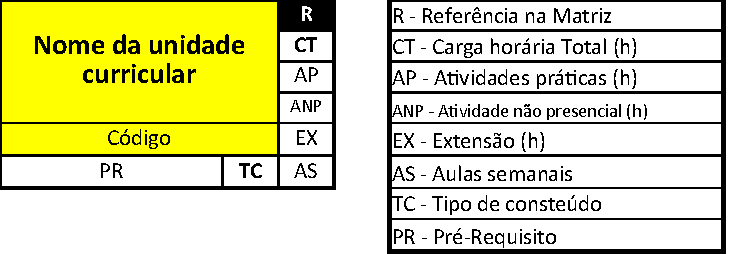
\includegraphics[width=0.6\textwidth]{Caps/Figs/Matriz_final_v2_leg.pdf}
	\fonte{\utf}
	\label{fig:legenda}
\end{figure}

\newgeometry{textwidth=200mm,textheight=290mm}
\begin{landscape}
	\begin{quadro}
		\centering
		\caption{Matriz do Curso de Engenharia Eletrônica}
		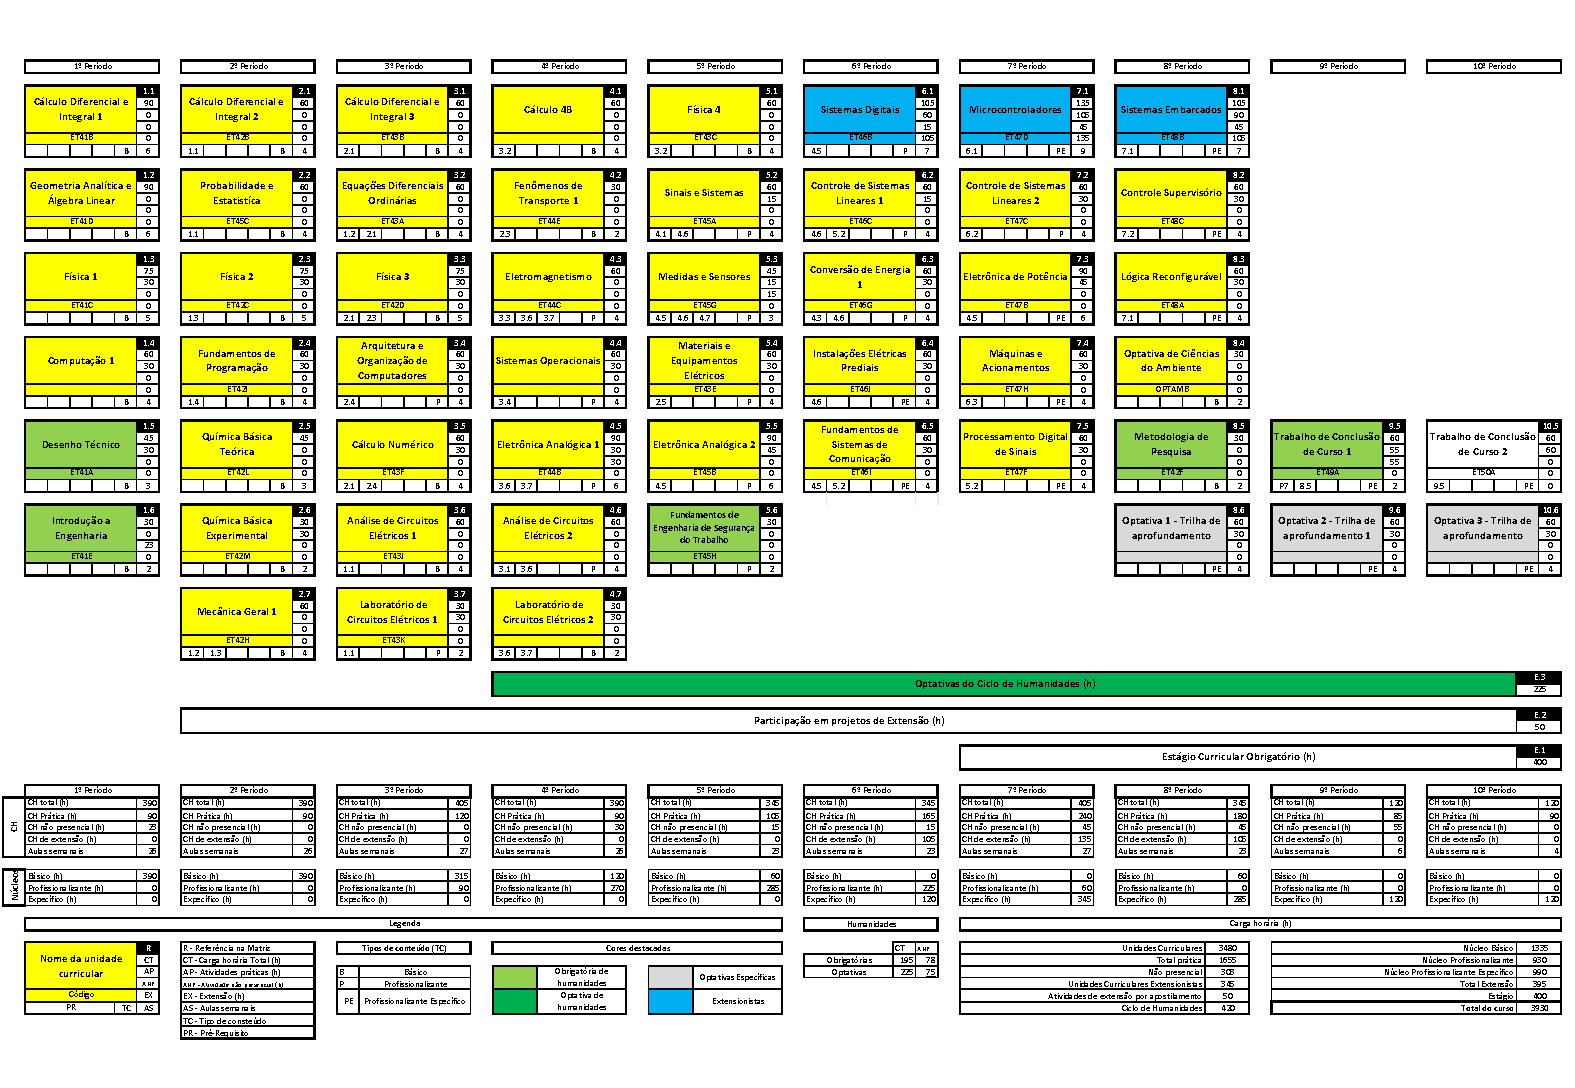
\includegraphics[width=1.3\textwidth]{Caps/Figs/Matriz_final_v2.pdf}
		\fonte{\utf}
		\label{qua:matriz}
	\end{quadro}
\end{landscape}
\restoregeometry



\subsection{Regime Letivo}
\label{sub:reg}

As atividades acadêmicas do curso são de regime semestral, com número mínimo de pré-requisitos, visando melhor consolidação dos conhecimentos nas áreas de atuação do engenheiro eletrônico. A matrícula no curso é realizada por Unidade Curricular. Quanto à matrícula e a periodização serão seguidas as normas institucionais do Regulamento de Organização Didático Pedagógica aplicável ao curso \cite{rodp}.

\subsection{Duração do curso}

O curso de Engenharia Eletrônica possui o período de integralização mínimo em 5 anos (10 períodos, sendo cada período equivalente a um semestre letivo) e máxima em 9 anos (18 semestres), de acordo com o Regulamento da Organização Didático Pedagógica dos Cursos de Graduação da UTFPR \cite{rodp}. A carga horária total é de \the\value{horasT} h. 

Destaca-se que, conforme a Instrução Normativa 02/10 da Instituição \cite{in2:2010:prograd}, uma aula na UTFPR possui 50 minutos. Assim sendo, cada hora das unidade curriculares correspondem a 1,2 aulas. Dessa forma, a cada 15 horas são realizadas 18 aulas.

\subsection{Carga horária de atividades teóricas e práticas}

As atividades teóricas (AT) do curso compreendem \the\value{horasAT} h, correspondendo a \percentagem{\the\value{horasAT}}{\the\value{horasT}} da carga horária total (\the\value{horasT} h). Conforme explicitado na \autoref{sec:matriz}, as ATs correspondem às atividades, de caráter presencial ou não, utilizadas para o desenvolvimento e compreensão de conceitos e de teorias.

\nomenclature[A]{PROGRAD}{Pró-reitoria de Graduação} 

As atividades práticas (AP) do curso compreendem \the\value{horasAP} h, correspondendo a \percentagem{\the\value{horasAP}}{\the\value{horasT}} da carga horária total (\the\value{horasT} h). São atividades de caráter presencial ou não, utilizadas para o desenvolvimento prático de conteúdos, tais como: atividades de laboratório, desenvolvimento de projetos, estudos de caso, visitas técnicas, levantamentos em campo, produção de textos, estágio, trabalho de conclusão de curso, atividades práticas de extensão, dentre outras. Além disso, todo ano é promovida a semana acadêmica com enfoque em atividades científicas, minicursos, atividades de extensão, palestras e seminários com profissionais que atuam em áreas pertinentes à formação do discente e outros. Também são promovidas, de acordo com a disponibilidade, visitas técnicas durante o curso.

\subsection{Carga horária de atividades não presenciais}

As atividades não presenciais (ANP) do curso compreendem \the\value{horasANP} h, correspondendo a \percentagem{\the\value{horasANP}}{\the\value{horasT}} da carga horária total (\the\value{horasT} h). As ANPs são distribuídas em diversas disciplinas estratégicas visando fomentar a cultura de ensino à distância no corpo discente e docente, gerando assim maturidade para esse processo de ensino-aprendizagem. Essa carga horária deve ser planejada pelos docentes, observando, necessariamente, a mediação por Tecnologias da Informação e Comunicação (TICS), assim como atender a regulamentação definida na Resolução nº 39/2019 – COGEP \cite{cogep39}. 

Segundo portaria de MEC N\textordmasculine{} 2.117, de 6 de dezembro de 2019 \cite{portaria2117mec}, as instituições de ensino poderão ofertar disciplinas em no máximo 40\% de sua carga horária total do curso. A principal ferramenta de Tecnologia de informação e comunicação (TIC) para a oferta desta modalidade é o sistema MOODLE. Para que uma disciplina ocorra desta maneira deve estar previsto em plano de ensino e ser aprovado por colegiado competente. Entretanto, em caso de ausência do docente por motivo previsto ou não previsto (como acidentes, doenças, falecimentos, dentre outros) a aula pode ser antecipada ou reposta por meio de uma atividade não presencial a distância desde que seja aprovada pelo coordenador do curso conforme Resolução n\textordmasculine 084/17 do COGEP \cite{cogep84}.

\nomenclature[A]{AD}{Aulas à distência}
\nomenclature[A]{ANPD}{Atividades não presenciais}

\subsection{Carga horária do Estágio Curricular Obrigatório}

Segundo as Diretrizes Curriculares Nacionais dos Cursos de Graduação em Engenharia \cite{dcneng}, em seu artigo 11, ``a formação  do  engenheiro  inclui,  como  etapa  integrante da  graduação, as práticas reais, entre as quais o estágio curricular obrigatório sob supervisão direta do curso''. Aliado a essa diretriz, a UTFPR estabelece, na Resolução COGEP-UTFPR N\textordmasculine{} 142/2022, de 25 de fevereiro de 2022 \cite{cogep142}, que a carga horária mínima de estágio obrigatório para os cursos da UTFPR deve ser de no mínimo \the\value{horasEST}, sendo esse o mesmo valor adotado pelo curso de Engenharia Eletrônica.

\nomenclature[A]{COEMP}{Conselho de Ralações Empresariais e comunitárias}

%\subsection{Carga horária do TCC}

%O TCC tem uma carga total de 144 horas-aula, a carga horária é dividida igualmente nas disciplinas de TCC 1 e TCC 2.

%\subsection{Carga horária de Atividade complementares}

%\pdfmarkupcomment{Verificar se as Atividade complementares continuarão.}{segundo as DCNs, deve-se manter}

\subsection{Carga horária das Atividades de Extensão}
\label{sub:extch}

A curricularização da Extensão no curso, é desenvolvida como uma possibilidade de aplicação de um conjunto de conhecimentos desenvolvidos durante as atividades de ensino e pesquisa e ofertada para a comunidade universitária da UTFPR, à comunidade no entorno direto da Universidade e às regiões circunvizinhas.

As atividades de Extensão enfocam a observação da realidade, tratada com o objetivo de produzir impacto junto à comunidade visando o desenvolvimento regional sustentável. Estarão organizadas em torno de programas ou projetos, sendo incluídas no projeto individual de algumas disciplinas, totalizando \the\value{horasEXT} h, representando \percentagem{\the\value{horasEXT}}{\the\value{horasT}} da carga horária total do curso.

\subsection{Carga horária dos Núcleos de Conteúdos}

Conforme estabelece as Diretrizes Curriculares Nacionais para os cursos Engenharia, existem três núcleos de conteúdo: (i) Básicos; (ii) Profissionalizantes e (iii) Profissionalizantes Específicos. A carga horária desses núcleos no âmbito do curso de Engenharia Eletrônica é mostrada no \autoref{tab:nucleos}.

\begin{table}
	\centering
	\caption[Carga horária dos núcleos de conteúdo]{Carga horária dos núcleos de conteúdo}        
    \label{tab:nucleos}
	\begin{tabularx}{0.7\textwidth}{>{\centering\arraybackslash}X >{\centering\arraybackslash}X >{\centering\arraybackslash}X }\toprule
	\textbf{Núcleo}					& \textbf{Carga horária (h)}	& \textbf{\% da carga horária total}	\\ \midrule 
	Básico							& \the\value{horasB}			& \percentagem{\the\value{horasB}}{\the\value{horasT}}	\\ \rowcolor{gray!10}
	Profissionalizante				& \the\value{horasPR}			& \percentagem{\the\value{horasPR}}{\the\value{horasT}}	\\ 
	Profissionalizante Específico	& \the\value{horasPE}			& \percentagem{\the\value{horasPE}}{\the\value{horasT}}	\\ \bottomrule
	\end{tabularx}
\end{table}

\subsection{Carga horária do ciclo de humanidades}

A fim de contribuir para uma formação mais humanística de seus egressos, os Projetos Pedagógicos dos Cursos de graduação da UTFPR devem estabelecer em sua estrutura curricular um ciclo de humanidades \cite{cogep142}, compreendendo um mínimo de 10$\%$ da carga horária total de unidades curriculares. 

No curso de Engenharia Eletrônica o ciclo de humanidades é estabelecido em \the\value{horasH} h, correspondendo a \percentagem{\the\value{horasH}}{\the\value{horasT}} da carga horária total do curso, ou \percentagem{\the\value{horasH}}{\the\value{horasUC}} da carga horária de unidades curriculares. A estruturação do ciclo de humanidades é demonstrada nas seções \ref{subsec:humanidades} e \ref{subsec:opthumanidades}.

\section{CONTEÚDOS CURRICULARES}

Esta seção descreve os componentes curriculares por período, as unidades curriculares obrigatórias, optativas e eletivas, demonstrando a totalização das cargas horárias.  A composição da distribuição gradual dos períodos e áreas de conhecimento é apresentado em uma sequência didática lógica demonstrando a integração entre os componentes curriculares. Também é descrito como está estruturado o ciclo de humanidades (grupo de unidades curriculares da área de humanidades exigido pela Resolução N\textordmasculine{} 142 COGEP \cite{cogep142}).

\subsection{Unidades Curriculares do Primeiro Período}

Este período do curso, historicamente, apresenta-se como um dos semestres mais difíceis e desafiadores para o corpo discente. Isto pode estar relacionado ao próprio momento em que o discente se encontra, buscando se adaptar a uma nova realidade, muitas das vezes experimentando o conflito entre a gestão da liberdade pessoal e a necessidade de se disciplinar frente às atividades acadêmicas. Em outra perspectiva, a turma do Primeiro Período geralmente apresenta grande diversidade de cultura e formação básica, o que torna importante a implementação de momentos de nivelamento e ambientação que propiciem um melhor fluxo de desenvolvimento das disciplinas e, consequentemente, seu melhor aproveitamento.

Desta forma, o Primeiro Período possui disciplinas que buscam e ambientar o discente ao curso, tais como ``Introdução à Engenharia'' e ``Computação 1''.

Adicionalmente, este período é o início do alicerce para as fundamentações matemáticas necessárias para o bom engenheiro eletrônico. Essa fundamentação se estende até o quarto período onde, a partir de então, as unidades curriculares específicas e profissionalizantes se iniciam.

%As unidades curriculares do Primeiro Período são \listaUC{1}{Dados/unidadesCurriculares.csv}, totalizando \the\value{horasP1} h. A \autoref{tab:per1} representa a distribuição das unidades curriculares do primeiro período do curso de Engenharia Eletrônica. Dessa forma,\listaUC{1}{Dados/unidadesCurriculares.csv}, totalizam \the\value{horasP1} h.

Os conteúdos curriculares do primeiro período estão listados na \autoref{tab:per1}. Adicionalmente, a estrutura de cada unidade curricular é apresentada em quadros: \listaUC{1}{Dados/unidadesCurriculares.csv}.

% tabela de unidades curriculares do primeiro período
\begin{table}[!htb]
	\centering\footnotesize
	\caption{Conteúdos curriculares do Primeiro Período}
	\label{tab:per1}
	\tabelaPeriodo{1}{Dados/unidadesCurriculares.csv}
	\fonte{Autoria própria}
\end{table}

\imprimeEmentas{1}{Dados/unidadesCurriculares.csv}\clearpage



\subsection{Unidades Curriculares do Segundo Período}

Os conteúdos curriculares do segundo período estão listados na \autoref{tab:per2}. Adicionalmente, a estrutura de cada unidade curricular é apresentada em quadros: \listaUC{2}{Dados/unidadesCurriculares.csv}.

% tabela de unidades curriculares do segundo período
\begin{table}[!htb]
	\centering\footnotesize
	\caption{Conteúdos curriculares do Segundo Período}
	\label{tab:per2}
	\tabelaPeriodo{2}{Dados/unidadesCurriculares.csv}
	\fonte{Autoria própria}
\end{table}

\imprimeEmentas{2}{Dados/unidadesCurriculares.csv}\clearpage

\subsection{Unidades Curriculares do Terceiro Período}

Os conteúdos curriculares do terceiro período estão listados na \autoref{tab:per3}. Adicionalmente, a estrutura de cada unidade curricular é apresentada em quadros: \listaUC{3}{Dados/unidadesCurriculares.csv}.

% tabela de unidades curriculares do terceiro período
\begin{table}[!htb]
	\centering\footnotesize
	\caption{Conteúdos curriculares do Terceiro Período}
	\label{tab:per3}
	\tabelaPeriodo{3}{Dados/unidadesCurriculares.csv}
	\fonte{Autoria própria}
\end{table}

\imprimeEmentas{3}{Dados/unidadesCurriculares.csv}\clearpage

\subsection{Unidades Curriculares do Quarto Período}

Os conteúdos curriculares do quarto período estão listados na \autoref{tab:per4}. Adicionalmente, a estrutura de cada unidade curricular é apresentada em quadros: \listaUC{4}{Dados/unidadesCurriculares.csv}.

% tabela de unidades curriculares do quarto período
\begin{table}[!htb]
	\centering\footnotesize
	\caption{Conteúdos curriculares do Quarto Período}
	\label{tab:per4}
	\tabelaPeriodo{4}{Dados/unidadesCurriculares.csv}
	\fonte{Autoria própria}
\end{table}

\imprimeEmentas{4}{Dados/unidadesCurriculares.csv}\clearpage

\subsection{Unidades Curriculares do Quinto Período}

Os conteúdos curriculares do quinto período estão listados na \autoref{tab:per5}. Adicionalmente, a estrutura de cada unidade curricular é apresentada em quadros: \listaUC{5}{Dados/unidadesCurriculares.csv}.

% tabela de unidades curriculares do quinto período
\begin{table}[!htb]
	\centering\footnotesize
	\caption{Conteúdos curriculares do Quinto Período}
	\label{tab:per5}
	\tabelaPeriodo{5}{Dados/unidadesCurriculares.csv}
	\fonte{Autoria própria}
\end{table}

\imprimeEmentas{5}{Dados/unidadesCurriculares.csv}\clearpage

\subsection{Unidades Curriculares do Sexto Período}

Os conteúdos curriculares do sexto período estão listados na \autoref{tab:per6}. Adicionalmente, a estrutura de cada unidade curricular é apresentada em quadros: \listaUC{6}{Dados/unidadesCurriculares.csv}.

% tabela de unidades curriculares do sexto período
\begin{table}[!htb]
	\centering\footnotesize
	\caption{Conteúdos curriculares do Sexto Período}
	\label{tab:per6}
	\tabelaPeriodo{6}{Dados/unidadesCurriculares.csv}
	\fonte{Autoria própria}
\end{table}

\imprimeEmentas{6}{Dados/unidadesCurriculares.csv}\clearpage

\subsection{Unidades Curriculares do Sétimo Período}

Os conteúdos curriculares do sétimo período estão listados na \autoref{tab:per7}. Adicionalmente, a estrutura de cada unidade curricular é apresentada em quadros: \listaUC{7}{Dados/unidadesCurriculares.csv}.

% tabela de unidades curriculares do sétimo período
\begin{table}[!htb]
	\centering\footnotesize
	\caption{Conteúdos curriculares do Sétimo Período}
	\label{tab:per7}
	\tabelaPeriodo{7}{Dados/unidadesCurriculares.csv}
	\fonte{Autoria própria}
\end{table}

\imprimeEmentas{7}{Dados/unidadesCurriculares.csv}\clearpage

\subsection{Unidades Curriculares do Oitavo Período}

Os conteúdos curriculares do oitavo período estão listados na \autoref{tab:per8}. Adicionalmente, a estrutura de cada unidade curricular é apresentada em quadros: \listaUC{8}{Dados/unidadesCurriculares.csv}.

% tabela de unidades curriculares do oitavo período
\begin{table}[!htb]
	\centering\footnotesize
	\caption{Conteúdos curriculares do Oitavo Período}
	\label{tab:per8}
	\tabelaPeriodo{8}{Dados/unidadesCurriculares.csv}
	\fonte{Autoria própria}
\end{table}

\imprimeEmentas{8}{Dados/unidadesCurriculares.csv}\clearpage

\subsection{Unidades Curriculares do Nono Período}

Os conteúdos curriculares do nono período estão listados na \autoref{tab:per9}. Adicionalmente, a estrutura de cada unidade curricular é apresentada em quadros: \listaUC{9}{Dados/unidadesCurriculares.csv}.

% tabela de unidades curriculares do nono período
\begin{table}[!htb]
	\centering\footnotesize
	\caption{Conteúdos curriculares do Nono Período}
	\label{tab:per9}
	\tabelaPeriodo{9}{Dados/unidadesCurriculares.csv}
	\fonte{Autoria própria}
\end{table}

\imprimeEmentas{9}{Dados/unidadesCurriculares.csv}\clearpage

\subsection{Unidades Curriculares do Décimo Período}

Os conteúdos curriculares do décimo período estão listados na \autoref{tab:per10}. Adicionalmente, a estrutura de cada unidade curricular é apresentada em quadros: \listaUC{10}{Dados/unidadesCurriculares.csv}.

% tabela de unidades curriculares do décimo período
\begin{table}[!htb]
	\centering\footnotesize
	\caption{Conteúdos curriculares do Décimo Período}
	\label{tab:per10}
	\tabelaPeriodo{10}{Dados/unidadesCurriculares.csv}
	\fonte{Autoria própria}
\end{table}

\imprimeEmentas{10}{Dados/unidadesCurriculares.csv}\clearpage

O Décimo período, assim como o nono, foram concebidos com poucas unidades curriculares (semipresenciais da trilha de aprofundamento), para que o discente possa finalizar o TCC, realizar o Estágio Curricular Obrigatório e integralizar as atividades de extensão.

O curso apresenta um máximo de \the\value{horasANP} horas em carga horária não presencial, distribuídas em diversas disciplinas. Essa carga horária deve ser planejada pelos docentes, observando, necessariamente, a mediação por Tecnologias da Informação e Comunicação (TICS), assim como atender a regulamentação definida na Resolução n\textordmasculine{} 39/2019 – COGEP \cite{cogep39}. A estratégia adotada contempla a combinação de ambientes físicos com ambientes digitais de aprendizagem, focados no desenvolvimento de projetos ou trabalhos práticos.

\subsection{Unidades Curriculares Optativas - Ciências do Ambiente}

O discente matriculado no curso de Engenharia Eletrônica deve cursar no mínimo 30 h de unidades curriculares de Ciências Ambientais. As unidades curriculares optativas de Ciências Ambientais estão listadas na \autoref{tab:per41}. Adicionalmente, a estrutura de cada unidade curricular é apresentada em quadros: \listaUC{41}{Dados/unidadesCurriculares.csv}. %Os dados estruturais das unidades curriculares estão nos quandros \ref{qua:ucCA78A}, \ref{qua:ucCA78B} e \ref{qua:ucCA78C}.

\begin{table}[!htb]
	\centering\footnotesize
	\caption{Conteúdos curriculares de Ciências Ambientais}
	\label{tab:per41}
	\tabelaTrilha{41}{Dados/unidadesCurriculares.csv}
	\fonte{Autoria própria}
\end{table}

\imprimeEmentasOpt{41}{Dados/unidadesCurriculares.csv}\clearpage



\subsection{Unidades Curriculares Optativas - Trilhas}
\label{subsec:trilhas}

As Trilhas de Aprofundamento foram concebidas como fator para flexibilização da matriz curricular, facilitador da mobilidade acadêmica e internacionalização e desenvolvimento de áreas de aprofundamento estratégicas para o curso, que foram escolhidas para atender o arranjo produtivo regional, bem como sintonizar a formação com o contexto tecnológico contemporâneo.

% Trilha de Controle e Automação
\subsubsection{Trilha de Controle e Automação}

Os conteúdos curriculares da Trilha de Controle e Automação estão listados na \autoref{tab:per21}. Adicionalmente, a estrutura de cada unidade curricular é apresentada em quadros: \listaUC{21}{Dados/unidadesCurriculares.csv}.

% tabela de unidades curriculares da Trilha de Controle e Automação
\begin{table}[!htb]
	\centering\footnotesize
	\caption{Conteúdos curriculares da trilha de Controle e Automação}
	\label{tab:per21}
	\tabelaTrilha{21}{Dados/unidadesCurriculares.csv}
	\fonte{Autoria própria}
\end{table}

\imprimeEmentasOpt{21}{Dados/unidadesCurriculares.csv}\clearpage

% Trilha de Computação
\subsubsection{Trilha de Computação}

Os conteúdos curriculares da Trilha de Computação estão listados na \autoref{tab:per22}. Adicionalmente, a estrutura de cada unidade curricular é apresentada em quadros: \listaUC{22}{Dados/unidadesCurriculares.csv}.

% tabela de unidades curriculares da Trilha de Computação
\begin{table}[!htb]
	\centering\footnotesize
	\caption{Conteúdos curriculares da trilha de Computação}
	\label{tab:per22}
	\tabelaTrilha{22}{Dados/unidadesCurriculares.csv}
	\fonte{Autoria própria}
\end{table}

\imprimeEmentasOpt{22}{Dados/unidadesCurriculares.csv}\clearpage

% Trilha de Eletrônica
\subsubsection{Trilha de Eletrônica}

Os conteúdos curriculares da Trilha de Eletrônica estão listados na \autoref{tab:per23}. Adicionalmente, a estrutura de cada unidade curricular é apresentada em quadros: \listaUC{23}{Dados/unidadesCurriculares.csv}.

% tabela de unidades curriculares da Trilha de Eletrônica
\begin{table}[!htb]
	\centering\footnotesize
	\caption{Conteúdos curriculares da trilha de Eletrônica}
	\label{tab:per23}
	\tabelaTrilha{23}{Dados/unidadesCurriculares.csv}
	\fonte{Autoria própria}
\end{table}

\imprimeEmentasOpt{23}{Dados/unidadesCurriculares.csv}\clearpage

% Trilha de Eletrotécnica
\subsubsection{Trilha de Eletrotécnica}

Os conteúdos curriculares da Trilha de Eletrotécnica estão listados na \autoref{tab:per24}. Adicionalmente, a estrutura de cada unidade curricular é apresentada em quadros: \listaUC{24}{Dados/unidadesCurriculares.csv}.

% tabela de unidades curriculares da Trilha de Eletrotécnica
\begin{table}[!htb]
	\centering\footnotesize
	\caption{Conteúdos curriculares da trilha de Eletrotécnica}
	\label{tab:per24}
	\tabelaTrilha{24}{Dados/unidadesCurriculares.csv}
	\fonte{Autoria própria}
\end{table}

\imprimeEmentasOpt{24}{Dados/unidadesCurriculares.csv}\clearpage

\subsection{O ciclo de Humanidades}
\label{subsec:humanidades}

De acordo com a Resolução COGEP/UTFPR N\textordmasculine{} 142, de 25 de fevereiro de 2022 \cite{cogep142}:

\begin{citacao}
	``os PPCs de graduação da UTFPR devem estabelecer em sua estrutura curricular, a partir do disposto nas DCNs, um ciclo de humanidades, representando uma carga horária igual ou superior a 10$\%$ (dez por cento) da carga horária total destinada às unidades curriculares do curso.''

\end{citacao}

Ainda segundo a referida Resolução: 

\begin{citacao}
	``o ciclo de humanidades será composto pelas áreas de ciências humanas, pela área de ciências sociais aplicadas e pela área de linguística, letras e artes, podendo incluir também, unidades/componentes curriculares na área de atividade física, saúde e qualidade de vida.''
\end{citacao}

Para a composição do ciclo de humanidades, a Resolução COGEP/UTFPR N\textordmasculine{} 142 estabelece os seguintes componentes:

\begin{enumerate}
	\item componentes da área de ciências humanas: antropologia, arqueologia, educação, filosofia, geografia, história, psicologia, sociologia, ciência política, relações internacionais e teologia, incluindo suas subáreas;
	\item componentes da área de ciências sociais aplicadas: administração, arquitetura e urbanismo, ciência da informação, direito, economia, planejamento urbano e regional, demografia, serviço social, turismo, desenho industrial, museologia e comunicação, incluindo suas subáreas;
	\item componentes da área de linguística, letras e artes: linguística, letras e artes, incluindo suas subáreas; e
	\item IV - atividade física, saúde e qualidade de vida.
\end{enumerate}

Dessa forma, o curso de Engenharia Eletrônica contempla em sua matriz um ciclo de humanidades composto por unidades curriculares obrigatórias e optativas, que representam \percentagem{\the\value{horasH}}{\the\value{horasUC}} da carga horária de unidades curriculares do curso. 


\subsection{Unidades Curriculares do Ciclo de Humanidades}
\label{subsec:obghumanidades}

A \autoref{tab:obghum}, mostra a relação das unidades curriculares obrigatórias do ciclo de humanidades junto com as respectivas áreas estabelecidas na Resolução COGEP/UTFPR N\textordmasculine{} 142 \cite{cogep142}. Também mostra, o quantitativo de carga horária de unidades curriculares optativas.

% tabela de unidades curriculares optativas de humanidades
\begin{table}[!htb]
	\centering\footnotesize
	\caption{Unidades curriculares de humanidades}
	\label{tab:obghum}
	\tabelaHum{Dados/unidadesCurriculares.csv}
	\fonte{Autoria própria}
\end{table}

\subsection{Unidades Curriculares Optativas do Ciclo de Humanidades}
\label{subsec:opthumanidades}

Os conteúdos curriculares optativos de Humanidades estão listados na \autoref{qua:ucHUM}, juntamente com as respectivas áreas estabelecidas na Resolução COGEP/UTFPR N\textordmasculine{} 142 \cite{cogep142}. Adicionalmente, a estrutura de cada unidade curricular é apresentada em quadros: \listaUC{31}{Dados/unidadesCurriculares.csv}.

% tabela de unidades curriculares optativas de humanidades
\begin{table}[!htb]
	\centering\footnotesize
	\caption{Conteúdos curriculares optativos de humanidades}
	\label{qua:ucHUM} % Não alterar
	\tabelaOptHum{31}{Dados/unidadesCurriculares.csv}
	\fonte{Autoria própria}
\end{table}

Para integralizar o ciclo de humanidades, o discente matriculado no curso de Engenharia Eletrônica deve cursar no mínimo 90 h da área de linguística e letras e 135 h nas demais áreas.

\imprimeEmentasHum{31}{Dados/unidadesCurriculares.csv}\clearpage


\section{O Estágio Curricular Obrigatório}

O Estágio Curricular Supervisionado deve oferecer condições suficientes para que o aluno possa, de acordo com o PDI \cite{pdiutfpr}, inserir-se com maior facilidade no mercado de trabalho. O PDI destaca:

\begin{citacao}
	``o estágio curricular é obrigatório para todos os cursos de nível técnico e de graduação, visa à complementação do processo ensino-aprendizagem e tem como objetivos: (i) facilitar a futura inserção do estudante no mundo de trabalho; (ii) servir como mecanismo de relacionamento entre a UTFPR e as entidades concedentes de estágio; e (iii) propiciar a adaptação social e psicológica do estudante à futura atividade profissional''.
\end{citacao}

%\dadoCHT{E.1}

O estágio como previsto na Lei nº 11.788, de 25 de setembro de 2008 \cite{Lei:11788:2008} é o ato educativo escolar supervisionado, desenvolvido no ambiente de trabalho, no qual visa a preparação do estudante para o ingresso no mercado de trabalho, facilitando a adaptação social e psicológica à futura atividade profissional do estudante. Além disso, busca-se o aprendizado de competências próprias da atividade profissional e a contextualização curricular, objetivando o desenvolvimento do educando para a vida cidadã e para o trabalho.

O estágio poderá ser realizado em organizações públicas, privadas ou do terceiro setor, que apresentem condições de proporcionar experiência prática na área de formação do estudante, podendo, também, proporcionar o desenvolvimento sócio cultural ou científico, pela participação em situações de vida e de trabalho no seu meio. O estágio pode ser realizado de duas formas:

\begin{itemize}
	\item Estágio Curricular Obrigatório: é aquele definido como tal no PPC, cuja carga horária é requisito para aprovação e obtenção de diploma;
	\item Estágio Não Obrigatório: é aquele desenvolvido como atividade opcional, acrescida à carga horária regular e obrigatória.
\end{itemize}

O Estágio Curricular Obrigatório é considerado disciplina/unidade curricular obrigatória dos cursos regulares do Ensino Superior da UTFPR. O Estágio Curricular Obrigatório deve ser planejado, executado, acompanhado e avaliado em conformidade com os currículos, programas e calendários acadêmicos. Poderá ser matriculado na disciplina/unidade curricular de Estágio Curricular Obrigatório o estudante que estiver regularmente matriculado na UTFPR a partir do 7\textordmasculine{} (sétimo) período do curso.

O Estágio Curricular Obrigatório tem duração mínima de \dadoCHT{E.1} h, podendo ser desenvolvido em mais de uma Unidade Concedente de Estágio (UCE), sendo que a atuação do estudante em cada uma delas não deverá ser inferior a 100 h. A jornada diária do estágio será compatível com o horário escolar do estudante, devendo constar no termo de compromisso e não ultrapassar 6 h diárias e 30 h semanais. Adicionalmente, nos períodos em que não estão programadas aulas presenciais os alunos poderão realizar estágio com carga horária de até 8 h diárias e 40 h semanais. O acompanhamento das atividades do estagiário deve ser feito pela UCE por meio da indicação de um funcionário supervisor, com formação ou experiência na área; pelo professor responsável pela atividade de estágio (PRAE) e pelo professor orientador.

O estudante que exercer atividade profissional correlata ao seu curso na condição de empregado devidamente registrado, autônomo ou empresário, ou ainda atuando oficialmente em programas de incentivo à pesquisa científica, ao desenvolvimento tecnológico, poderá valer-se de tais atividades para efeitos de realização do seu Estágio Curricular Obrigatório, desde que atendam ao PPC.

As atividades de Estágio Não Obrigatório podem ser iniciadas a partir do segundo semestre e durante todo o curso, com exceção do período de realização do Estágio Curricular Obrigatório, através de convênios ou projetos firmados entre a Universidade e UCE. O Estágio será precedido da celebração do instrumento jurídico entre o estudante e a UCE, com interveniência da UTFPR, por meio da Diretoria de Relações Empresariais e Comunitárias (DIREC).

Os procedimentos para a realização e acompanhamento de estágios nos Cursos de Educação Profissional Técnica de Nível Médio e no Ensino Superior da UTFPR são estabelecidos pela Resolução Conjunta N\textordmasculine{} 01/2020, de 02 de junho de 2020 \cite{cogepcoemp1:2020}.

% Colocar a norma do curso assim que for publicada

\section{Trabalho de conclusão de curso}

O Trabalho de Conclusão de Curso (TCC) é um componente curricular obrigatório para os cursos de graduação \cite{dcneng}. No ambito da UTFPR, o TCC deve atender à resolução n\textordmasculine 18/2018 – COGEP, Regulamento do Trabalho de Conclusão de Curso (TCC) para os Cursos de Graduação da UTFPR \cite{cogep18}. Os objetivos do TCC são:

\begin{enumerate}
	\item Desenvolver a capacidade de aplicação dos conceitos e teorias adquiridas durante o curso de forma integrada;
	\item Desenvolver a capacidade de planejamento e disciplina para resolver problemas dentro das diversas áreas de formação;
	\item Despertar o interesse pela aplicação do conhecimento como meio para a resolução de problemas;
	\item Estimular o espírito empreendedor, por meio de desenvolvimento de projetos;
	\item Intensificar a extensão universitária, por intermédio da resolução de problemas e identificação de oportunidades existentes nos diversos setores da sociedade;
	\item Desenvolver a capacidade de análise e de busca de soluções para problemas sociais, políticos, tecnológicos, ambientais, éticos e metodológicos;
	\item Estimular a construção do conhecimento coletivo; 
	\item Estimular a inter, multi e transdisciplinaridade;
	\item Estimular a inovação tecnológica, através da transferência de tecnologia, desenvolvimento de patentes e/ou comercialização dos resultados;
	\item Estimular a articulação entre ensino e pesquisa.  
		
\end{enumerate}

O TCC está dividido em duas etapas: TCC 1 e TCC 2, onde cada etapa contempla 60 h. O objetivo final no TCC 1 é a elaboração de um projeto de pesquisa e defendê-lo frente a uma banca avaliadora, incluindo o professor orientador. O TCC 2 tem como objetivo a execução desse projeto de pesquisa e sua defesa pública, conforme regulamento acima citado e normas complementares de TCC do curso de Engenharia Eletrônica campus Toledo, aprovadas em colegiado.

As atividades de TCC do curso são coordenadas por um Professor Responsável pela atividade de TCC (PRATCC) indicado pelo coordenador do curso. Cabe a esse professor constituir as bancas de avaliação e apoiar as diversas atividades relativas a TCC. O acompanhamento dos alunos no TCC é efetuado por um Professor Orientador, indicado pelo Professor Responsável pelo TCC. O detalhamento das atividades de TCC, bem como das responsabilidades dos envolvidos, podem ser obtidas na norma geral de TCC da UTFPR \cite{cogep18}.

\section{Síntese de distribuição de carga horária}

A \autoref{tab:ch} sumariza as cargas horárias do curso, indicando os totais para o Ciclo de Humanidades, atividades de extensão, TCC e para as atividades não presenciais. Os percentuais de cada total é calculado em relação a carga horária total do curso (\the\value{horasT} h).

É possível notar, através da referida tabela, que o curso atende à Resolução CNE/CES N\textordmasculine{} 7, de 18 de dezembro de 2018, que determina um mínimo de 10$\%$ da carga horária do curso, voltada para atividades extensionistas.

\begin{table}[!htb]
	\rowcolors{3}{white}{tableShade}
	\centering
	\caption{Síntese de distribuição de carga horária do curso de Engenharia Eletrônica}
	\label{tab:ch}
	\begin{tabularx}{\textwidth}{c|>{\centering\arraybackslash}X | >{\centering\arraybackslash}X | c} \toprule%\hiderowcolors
		\bfseries Item		& \bfseries Atividade										& \bfseries Carga Horária (h) 	&	\bfseries Composição$^1$	\\	\midrule \midrule
		a = d + f + i		& Integralização / Carga horária Total						& \the\value{horasT}			&	100$\%$			\\			
		b					& Unidades Curriculares Optativas							& \the\value{horasOPT}			&	\percentagem{\the\value{horasOPT}}{\the\value{horasT}}				\\	
		c					& Unidades Curriculares Obrigatórias						& \the\value{horasOBG}			&	\percentagem{\the\value{horasOBG}}{\the\value{horasT}}				\\	
		d = c + d			& Unidades Curriculares										& \the\value{horasUC}			&	\percentagem{\the\value{horasUC}}{\the\value{horasT}}				\\	
		e					& Unidades Curriculares extensionistas						& \the\value{horasUCEXT}		&	\percentagem{\the\value{horasUCEXT}}{\the\value{horasT}}			\\	
		f					& Atividades extensionistas complementares / Apostilamento	& \the\value{horasCEXT}			&	\percentagem{\the\value{horasCEXT}}{\the\value{horasT}}				\\	
		g = e + f			& Atividades extensionistas 								& \the\value{horasEXT}			&	\percentagem{\the\value{horasEXT}}{\the\value{horasT}}				\\	
		h					& Ciclo de Humanidades 										& \the\value{horasH}			&	\percentagem{\the\value{horasH}}{\the\value{horasT}}$^2$				\\	
		i					& Estágio 													& \the\value{horasEST}			&	\percentagem{\the\value{horasEST}}{\the\value{horasT}}				\\	
		j					& Não presencial 											& \the\value{horasANP}			&	\percentagem{\the\value{horasANP}}{\the\value{horasT}}				\\	
		l					& Trabalho de Conclusão de Curso							& 120							&	\percentagem{120}{\the\value{horasT}}				\\	\bottomrule
		
	\end{tabularx}
	\begin{tabularx}{\textwidth}{l}
		\hiderowcolors
		\tiny $^1$ - Porcentagem em relação à carga horária Total\\
		\tiny $^2$ - Representa \percentagem{\the\value{horasH}}{\the\value{horasUC}} da carga horária das unidades curriculares.
	\end{tabularx}
\end{table}

Ademais, as diretrizes curriculares dos cursos de graduação regulares da UTFPR \cite{cogep142} determinam que os PPCs de cursos de graduação da UTFPR devem estabelecer em sua estrutura curricular, a partir do disposto nas DCNs \cite{dcneng}, o ciclo de humanidades, representando uma carga horária igual ou superior a 10$\%$ (dez por cento) da carga horária total destinada às unidades curriculares do curso. Dessa forma, o curso de Engenharia Eletrônica, estabelece \the\value{horasH} h de unidades curriculares humanísticas, representando \percentagem{\the\value{horasH}}{\the\value{horasUC}} da carga horária das unidades curriculares.

\section{Processo de ensino e aprendizagem}

O processo de como o docente trata o ensino e a aprendizagem relaciona-se com uma serie de questionamentos sobre a própria definição do que é aprender e ensinar. Dessa forma, é necessário que os educadores sejam capazes de entender as diferenças de cada atividade e procurar escolher a melhor maneira que irá desenvolver um determinado tema. 

\subsection{Metodologias de aprendizagem}

As metodologias de aprendizagem aplicada no curso de Engenharia Eletrônica são formas de organizar o ensino do discente visando obter o melhor desempenho para atingir o perfil do egresso. Trata-se do ``caminho'' a seguir para conseguir entender e internalizar todo o conhecimento passado. Dessa forma, as metodologias aplicadas estão intimamente relacionadas ao desenvolvimento das competências profissionais apresentadas na \autoref{sec:perf}. As competências são desenvolvidas gradativamente em várias unidades curriculares e em momentos distintos no decorrer do curso, assim como é explicado na \autoref{sec:comp}.

Ao docente atuante no curso de Engenharia Eletrônica é dada a liberdade da escolha da metodologia a ser empregada nas ações de ensino. Esse processo é acompanhado pelo NDE e pelo Departamento de Educação (DEPED-TD), sempre visando o melhor aproveitamento do discente. Neste sentido, a UTFPR dispõe de um Programa de Desenvolvimento Profissional Docente da UTFPR, aprovado pela Resolução COGEP N\textordmasculine{} 32/2019 \cite{cogep32}, com finalidade do aperfeiçoamento da prática docente, possibilitando a busca de alternativas às dificuldades que envolvem os processos de ensino e aprendizagem na Instituição.

São exemplos de metodologias que podem ser empregadas:

\begin{itemize}
	\item Metodologias ativas: o aluno é o principal responsável pelo aprendizado do conteúdo através da participação, interagindo e pensando para aumentar a absorção. Pode-se utilizar estudos de caso, projetos práticos e debates entre equipes de discentes. É o contrario da metodologia passiva, onde o discente apenas assiste as aulas expositivas e depois é avaliado através de provas e trabalhos;
	\item Método de aprendizagem interativo: existe iteração entre o aluno e objeto de estudo, prendendo a atenção do estudante e aprimorando o processo de aprendizagem, como é o caso dos jogos, desafios, animações e atividades práticas de laboratório;
	\item Método de autoaprendizagem: o discente tem liberdade nos estudos, sendo o responsável por gerir o tempo de dedicação na objeto estudado. A dependência de outros profissionais é minimizada, podendo existir a sugestão ou seleção de um bom material de ensino. Esse método é bastante comum nas práticas onde existe um docente orientador de projetos práticos, como é o caso de TCC, IC, IT e trabalhos extraclasse de disciplina.
\end{itemize}



\subsection{Tecnologias de Informação e Comunicação (TICs)}

A instituição disponibiliza alguns ambientes e artefatos de comunicação para mediarem atividades didáticas nas modalidades presencial e não presencial:

\begin{itemize}
    \item Página pessoal docente;
    \item Moodle institucional;
    \item Plataforma GSuite for Education;
    \item Serviço Mconf em parceria com a Rede Nacional de Ensino e Pesquisa (RNP);
    \item Base Digital de dados;
    \item Repositórios institucionais;
    \item Office 365;
    \item Equipamentos de áudio e vídeo em geral.
\end{itemize}
    
Diante disso, o processo de ensino aprendizagem é intensificado com o uso das TICs e demais artefatos tecnológicos, por meio de atividades de comunicação, colaboração e compartilhamento, propiciando a construção e a produção de conhecimentos e o desenvolvimento de habilidades pessoais e interpessoais do corpo discente, e fomentando novas práticas do docente.

Mais informação sobre a utilização de TICs nos processos de ensino e aprendizagem no ambito do curso de Engenharia Eletrônica podem ser encontrados na \autoref{sec:tic}.

\subsection{Processos de avaliação}

O Curso tem como horizonte formar pessoas com capacidade de se expressarem escrita e oralmente, que desenvolvam trabalhos em equipes multidisciplinares, que compreendam e utilizem novas ideias e tecnologias para a resolução de problemas, e os procedimentos de avaliação do processo de ensino-aprendizagem utilizados no curso partem desse pressuposto. São diversificados, elaborados de acordo com a especificidade de cada disciplina, buscando levar em consideração o profissional que se quer formar.

A avaliação do processo de ensino-aprendizagem parte dos objetivos das disciplinas e não negligencia instrumentos como provas escritas, trabalhos de pesquisa bibliográfica, produção de artigos, etc. Por outro lado, há o interesse que se desenvolva no interior das disciplinas, atividades que articulem diferentes áreas do curso, que busquem desenvolver materiais de trabalho que expressem a reflexão sobre problemáticas da sociedade, entre outras questões importantes para o profissional da área.

Mesmo com a realização das provas individuais busca-se diversificar, com a contribuição das Tecnologias de Informação e Comunicação – TICs. Estas podem ser utilizadas em disciplinas como a Estatística e Desenho Técnico, quando softwares computacionais são empregados para a resolução de questões; e a plataforma MOODLE como veículo para a realização de avaliações. A proposição de trabalhos de pesquisa sobre conteúdo específicos e sua formação em editores de texto é uma prática comum ao longo das disciplinas.

No entanto, o emprego de provas individuais para verificar se os objetivos da disciplina foram atingidos, é apenas um dos instrumentos utilizados para avaliar os discentes ao longo do curso e no interior das unidades curriculares. Há a preocupação em avaliar a capacidade do discente em desenvolver seus trabalhos com criatividade, autonomia, flexibilidade e conhecimento vinculando conteúdos para propiciar uma experiência multidisciplinar. 

Com essas estratégias, todas as unidades curriculares do curso utilizam diferentes instrumentos de avaliação, não se resumindo às provas escritas. Além disso, propicia que o acadêmico seja avaliado em diferentes momentos, ao mesmo tempo em que exige diversificados critérios de avaliação. 

Tentando contribuir para a concretização disso, há um cuidado na aprovação dos planos de ensino das unidades curriculares, para que elas expressem claramente os critérios e os instrumentos de avaliação utilizados. O docente da disciplina tem autonomia para estabelecer os pesos específicos para os diferentes instrumentos utilizados. No entanto, é incentivado pelo grupo a utilizar diferentes instrumentos e critérios de avaliação. 

A avaliação da aprendizagem dos discentes por componente curricular, levando-se em consideração a assiduidade e o aproveitamento nos estudos, é realizada de acordo com as especificações referidas no Regulamento da Organização Didático-Pedagógica dos Cursos de Graduação da UTFPR (Resolução n\textordmasculine{} 81/2019 - COGEP, de 26 de julho de 2019 \cite{rodp}) em seu capítulo VI (Do Ensino, do Rendimento escolar e da Aprovação) que segue as seguintes diretrizes: 

\begin{itemize}
	\item Avaliação: número de avaliações não menor do que 2 (duas), onde suas modalidades e critérios devem ser explicitados no Planejamento de Aulas da unidade curricular. Além disso, o docente deverá possibilitar a reavaliação ao longo e/ou ao final do semestre letivo a todos os estudantes matriculados na unidade curricular, oportunizando ao estudante alcançar nota final para aprovação.
	\item Aprovação: frequência igual ou superior a 75$\%$ (setenta e cinco por cento) das aulas presenciais dadas e Nota Final igual ou superior a 6,0 (seis), ou frequência igual ou superior a 50$\%$ (cinquenta por cento) das aulas presenciais dadas e Nota Final igual ou superior a 8,0 (oito);
	\item Aproveitamento: os alunos serão avaliados através de atividades que resultem na avaliação do conhecimento por atribuição de notas a critério do professor e segundo o plano de ensino da disciplina. A flexibilização do regimento da Instituição permite que o professor possa alterar os critérios propostos conforme a necessidade de cada disciplina;
	\item  Condições especiais: pela Resolução n\textordmasculine{} 110/2021 – COGEP \cite{cogep110}, tem-se também o regulamento que estabelece normas para as atividades de acompanhamento domiciliar, abono de faltas, compensação de faltas, dispensa de frequência e lançamento de faltas para os cursos presenciais de nível médio e superior da UTFPR em que situações diversas são consideradas permitindo uma melhor flexibilização do processo de avaliação discente.
\end{itemize}

\subsection{Avaliação dos discentes com necessidades especiais}

Os discentes com necessidades especiais apresentam características e particularidades que não podem ser tratadas e trabalhadas de maneira homogênea em seus aspectos cognitivos, físicos e psicossociais. São necessidades que requererem dos professores e da própria Universidade um tratamento diferenciado, levando em consideração os conceitos expressos pela Lei Brasileira de Inclusão da Pessoa com Deficiência (LBI) n\textordmasculine{} 13.146, de 06/07/2015, em seu artigo 3\textordmasculine{} que explicita e conceitua o que é acessibilidade, desenho universal, tecnologia assistiva, barreiras, comunicação, adaptações razoáveis, elemento de urbanização, mobiliário urbano, pessoa com mobilidade reduzida, residências inclusivas, moradia para a vida independente da pessoa com deficiência, atendente pessoal, profissional de apoio escolar e acompanhante.

A UTFPR campus Toledo conta em seu quadro funcional com um intérprete de libras, pedagogo, psicólogo, que atuam junto ao aluno com necessidades especiais ou com necessidades especiais de avaliação e a equipe docente.

Medidas para contribuir com a formação e atuação dos docentes com alunos com necessidades especiais são colocadas em prática para favorecer a melhoria dos processos de ensino e aprendizagem. Essas medidas envolvem desde o atendimento direto desses alunos e suas famílias no campus até o intercâmbio de informações com outras Universidades para implementação de propostas de políticas de inclusão, com atividades como leituras, debates, reflexões com textos e obras sobre inclusão pelos grupos de Estudo e Pesquisas do campus, monitorias com horários diferenciados para os alunos com necessidades especiais, previsto no Regulamento da Monitoria da UTFPR, adequação dos espaços físicos para os alunos com necessidades especiais, e acompanhamento de intérprete de Libras em sala de aula e nos atendimentos da monitoria.

   % Matriz curricular
    
    
    
    % Bibliografia
    \bibliography{references}
    
    \postextual
    
    % Apêndices:
    \apendices
    %\chapter{Apêndice 1}
\label{apen:apen1}

\lipsum
    
    % Anexos:
    \anexos
    %\chapter{Anexo 1}
\label{anex:anex1}

\lipsum
    
\end{document}
